% Diese Datei repräsentiert den Inhalt der Präsentation

% Titelseite
\begin{frame}[t,plain]
    \titlepage
\end{frame}

% table of contents
\section{Innføring}
\subsection*{Agenda}
\begin{frame}
    \tableofcontents
\end{frame}

\subsection*{Download PDFen}
\begin{frame}{Last meg ned}
    \begin{figure}
        \centering
        
\includegraphics[height = 4.9cm]{images/downloadqr.png}
        \caption{https://tinyurl.com/inf115v22}
        \label{fig:qrcode}
    \end{figure}
\end{frame}

\section{SQL}
\subsection*{Teamer}
\begin{frame}{Temaer}
\begin{itemize}
    \item Select
    \item Aggregation
    \item Joins
    \item Update
    \item Insert
    \item Delete
    \item Create and Drop Tables
    \item Datatyper
    \item Constraints
    \item Alt mulig
\end{itemize}
\end{frame}

\subsection*{Enkle Select statements}
\begin{frame}[fragile]{Select}
\begin{minted}{sql}
SELECT director, COUNT(*) as c -- Spalter
FROM movie                     -- Tabeller
WHERE country = "Dabendorf"    -- Betingelser
GROUP BY director              -- Gruppering etter spalter
HAVING c > 3                   -- Betingelser etter gruppering
ORDER BY c DESC                -- Sortering etter spalter 
LIMIT 3;                       -- Velg de første n output linjene
\end{minted}
\end{frame}

\subsection*{Aggregasjonsfunksjoner}
\begin{frame}[fragile]{Aggregation}
\begin{itemize}
    \item Count: Teller antall elementer
    \item Sum: Summerer verdier
    \item Avg: Gjennomsnitt av verdier (tilsvarer count/sum)
    \item Min: Minimum
    \item Max: Maksimum
    \item Alle aggregasjonsfunksjoner ignorerer NULL verdier
\end{itemize}
\end{frame}

\subsection*{Joins}
\begin{frame}[fragile]{Join (2 varianter)}
\begin{minted}{sql}
SELECT *                -- Variante 1
FROM film, screening    -- Velg alle tabeller og bruk WHERE
WHERE film.film_id = screening.film_id;
\end{minted}
\begin{minted}{sql}
SELECT *                -- Variante 2
FROM film               -- Velg en tabell og bruk JOIN og ON
JOIN screening ON film.film_id = screening.film_id;
\end{minted}
\end{frame}

\begin{frame}{Types of Joins}
\begin{itemize}
    \item INNER JOIN: Alle rad som finnes i begge tabeller
    \item LEFT (OUTER) JOIN: Alle rad som finnes i begge tabeller og alt fra venstre tabellen
    \item RIGHT (OUTER) JOIN: Alle rad som finnes i begge tabeller og alt fra høyre tabellen
    \item FULL (OUTER) JOIN: Alt fra begge tabeller
    \item \textit{Alt} mener tilsvarende JOIN columns
    \item Ikke-eksisterende verdier fylles med NULL verdier
    \item \dots SELF JOIN, CROSS JOIN, NATURAL JOIN, \dots
\end{itemize}
\end{frame}

\begin{frame}{Venn Diagram}
    \begin{figure}
        \centering
        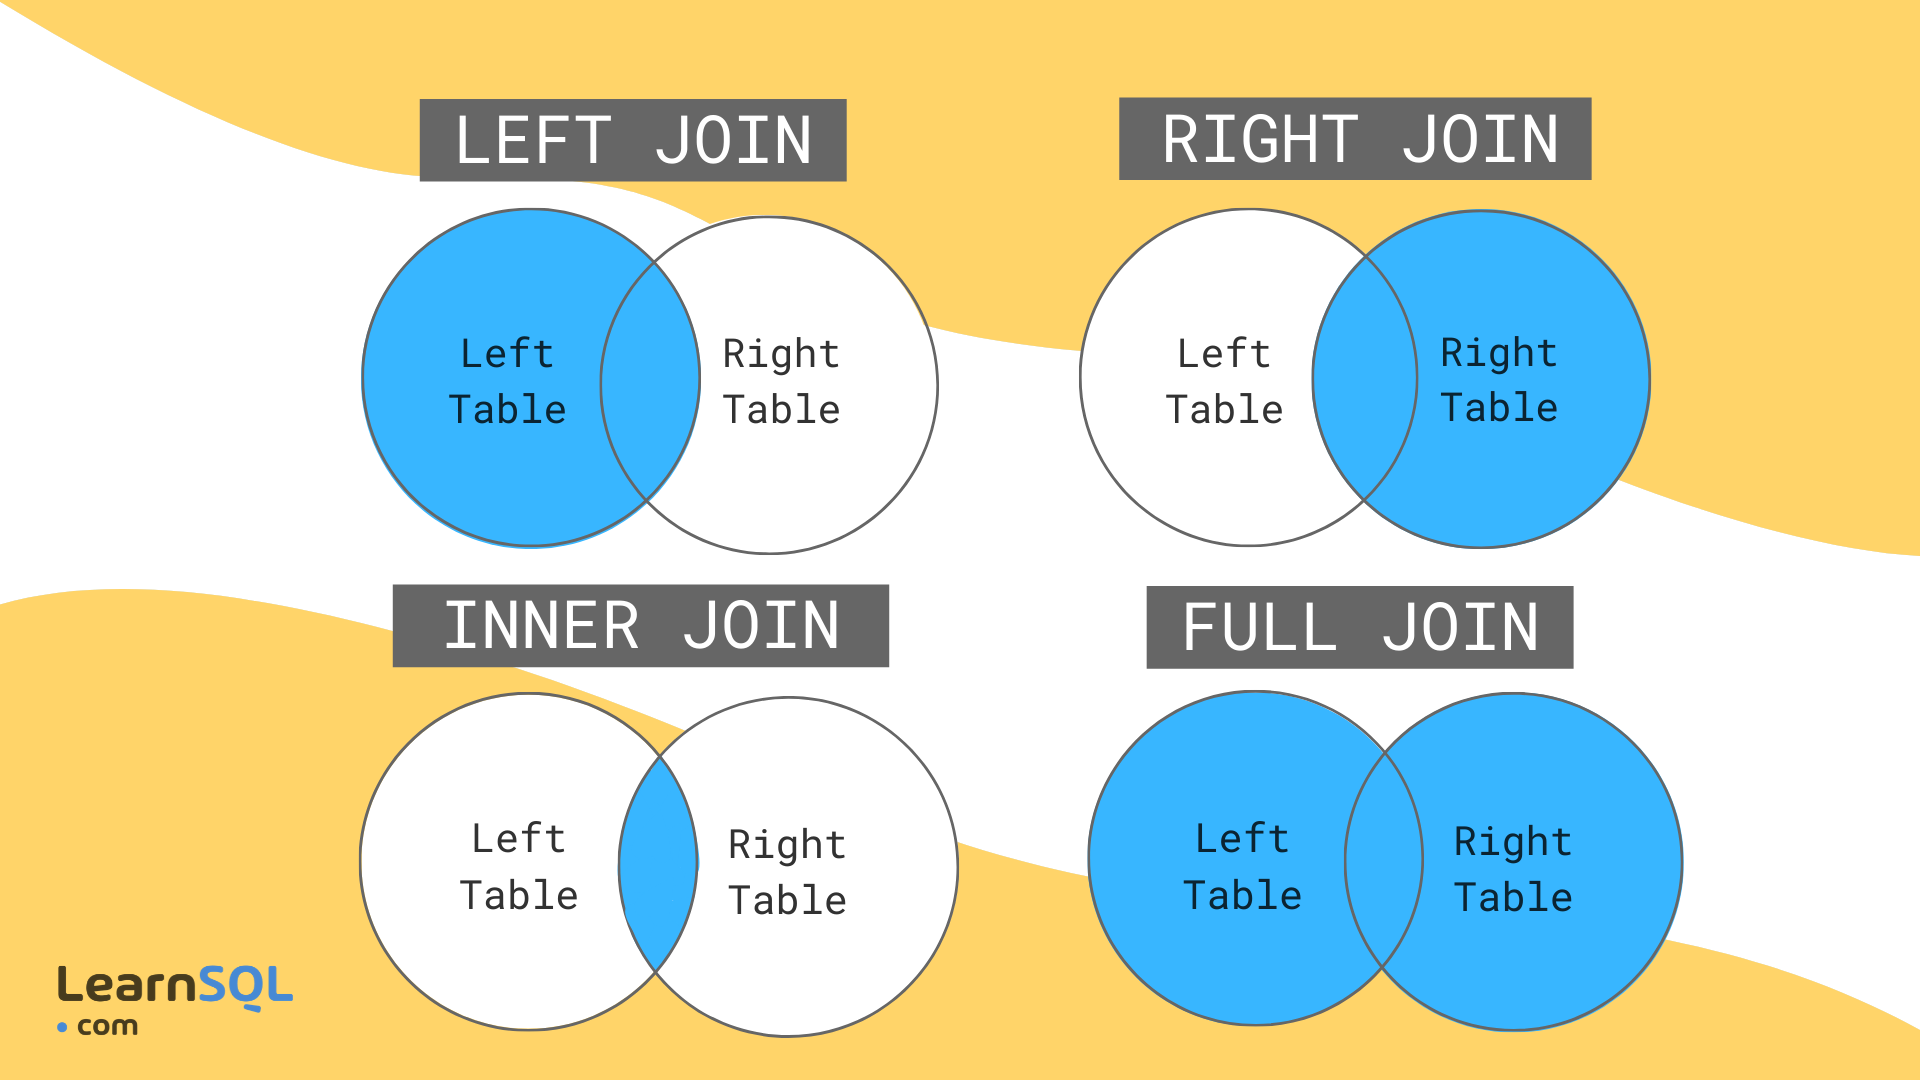
\includegraphics[height = 4.9cm]{images/joins.png}
        \caption{Kilde: https://learnsql.com/blog/learn-and-practice-sql-joins/}
        \label{fig:venndiagram}
    \end{figure}
\end{frame}

\subsection*{Oppdatere informasjoner}
\begin{frame}[fragile]{Update}
\begin{minted}{sql}
UPDATE book                 -- tabell
SET title = "Der satanarchäolügenialkohöllische Wunschpunsch"
WHERE book_id = 37;         -- betingelse
\end{minted}
\begin{minted}{sql}
UPDATE music                -- tabell
SET title = "Supercalifragilisticexpialidocious",
   artist = "Mary Poppins"  -- oppdatert informasjon
WHERE song_id = 42;         -- betingelse
\end{minted}
\end{frame}

\subsection*{Legg til informasjoner}
\begin{frame}[fragile]{Insert (2 varianter)}
\begin{minted}{sql}
INSERT INTO film (film_id, title, director, genre)
VALUES (7, "Fantômas", "André Hunebelle", "Fransk tull"); 
\end{minted}

\begin{minted}{sql}
INSERT INTO film    -- spaltenavn ikke nødvendig hvis alle blir brukt
VALUES (7, "Fantômas", "André Hunebelle", "Fransk tull"); 
\end{minted}
\end{frame}

\subsection*{Fjerne informasjoner}
\begin{frame}[fragile]{Delete}
\begin{minted}{sql}
DELETE FROM film        -- tabell
WHERE country = "USA";  -- betingelse
\end{minted}
\end{frame}

\subsection*{Lage nye tabeller}
\begin{frame}[fragile]{Create Table}
\begin{minted}{sql}
CREATE TABLE Persons (
    Person_id int,              -- column name, datatype
    LastName varchar(40) NOT NULL,
    FirstName varchar(40),
    Age int,
    Department_id int UNIQUE,
    PRIMARY KEY (Person_id),    -- primær- og fremmednøkler
    FOREIGN KEY (Department_id) REFERENCES Department(Department_id),
    CHECK (Age>=18)             -- constraints
);
\end{minted}
\end{frame}

\subsection*{Slette tabeller}
\begin{frame}[fragile]{Drop Table}
\begin{minted}{sql}
DROP TABLE eksamenskarakterer;  -- tabell som skal slettes 
\end{minted}
\end{frame}

\subsection*{Datatyper}
\begin{frame}[fragile]{Datatyper}
\begin{minted}{sql}
char(20)            -- 20 tegn med fast lengde
varchar(20)         -- opptil 20 tegn
text                -- tekst med opptil 2^16 tegn
int                 -- integer (tinyint, smallint, bigint)
float(2)            -- float med 2 sifre bak komma
decimal(5,2)        -- 3 sifre før og 2 etter komma
enum ("INF102", "INF234", "INF237") -- en av n verdier
date                -- dato
timestamp           -- unix timestamp
\end{minted}
\end{frame}

\subsection*{Constraints}
\begin{frame}[fragile]{Constraints}
\begin{minted}{sql}
NOT NULL                    -- verdien er ikke NULL
UNIQUE                      -- spalten har ingen verdi flere ganger
PRIMARY KEY(key)            -- NOT NULL + UNIQUE
FOREIGN KEY(key) REFERENCES tabell(key) -- fremmednøkkel
AGE int CHECK (AGE >= 18)   -- betingelse
AGE int DEFAULT 18          -- standardverdi
\end{minted}
\end{frame}

\subsection*{Andre ting}
\begin{frame}[fragile]{Alt mulig}
\begin{minted}{sql}
SELECT DISTINCT                     -- fjerner duplikater
WHERE navn LIKE "A\%"               -- alt som starter med A
-- \% 0, 1 eller flere tegn
-- _ eksakt et tegn
WHERE category IN ("cake", "bread") -- verdien er i en liste
WHERE age BETWEEN 18 and 65         -- verdien er i en range
WHERE EXISTS (SELECT ...)           -- verdien finnes i en annen query
(SELECT ...) UNION (SELECT ...)     -- union av to queries
\end{minted}
\end{frame}

\begin{frame}[fragile]{Alt mulig}
\begin{minted}{sql}
SELECT Order_id, Price,
CASE    -- if betingelser i SELECT
    WHEN Price > 30 THEN "Won't pay freight"
    ELSE "Freight costs 10\$"
END AS FrightCost
FROM OrderDetails; 
\end{minted}
\end{frame}

\subsection*{Spørretid}
\begin{frame}{Spørsmål?}
    \begin{figure}
        \centering
        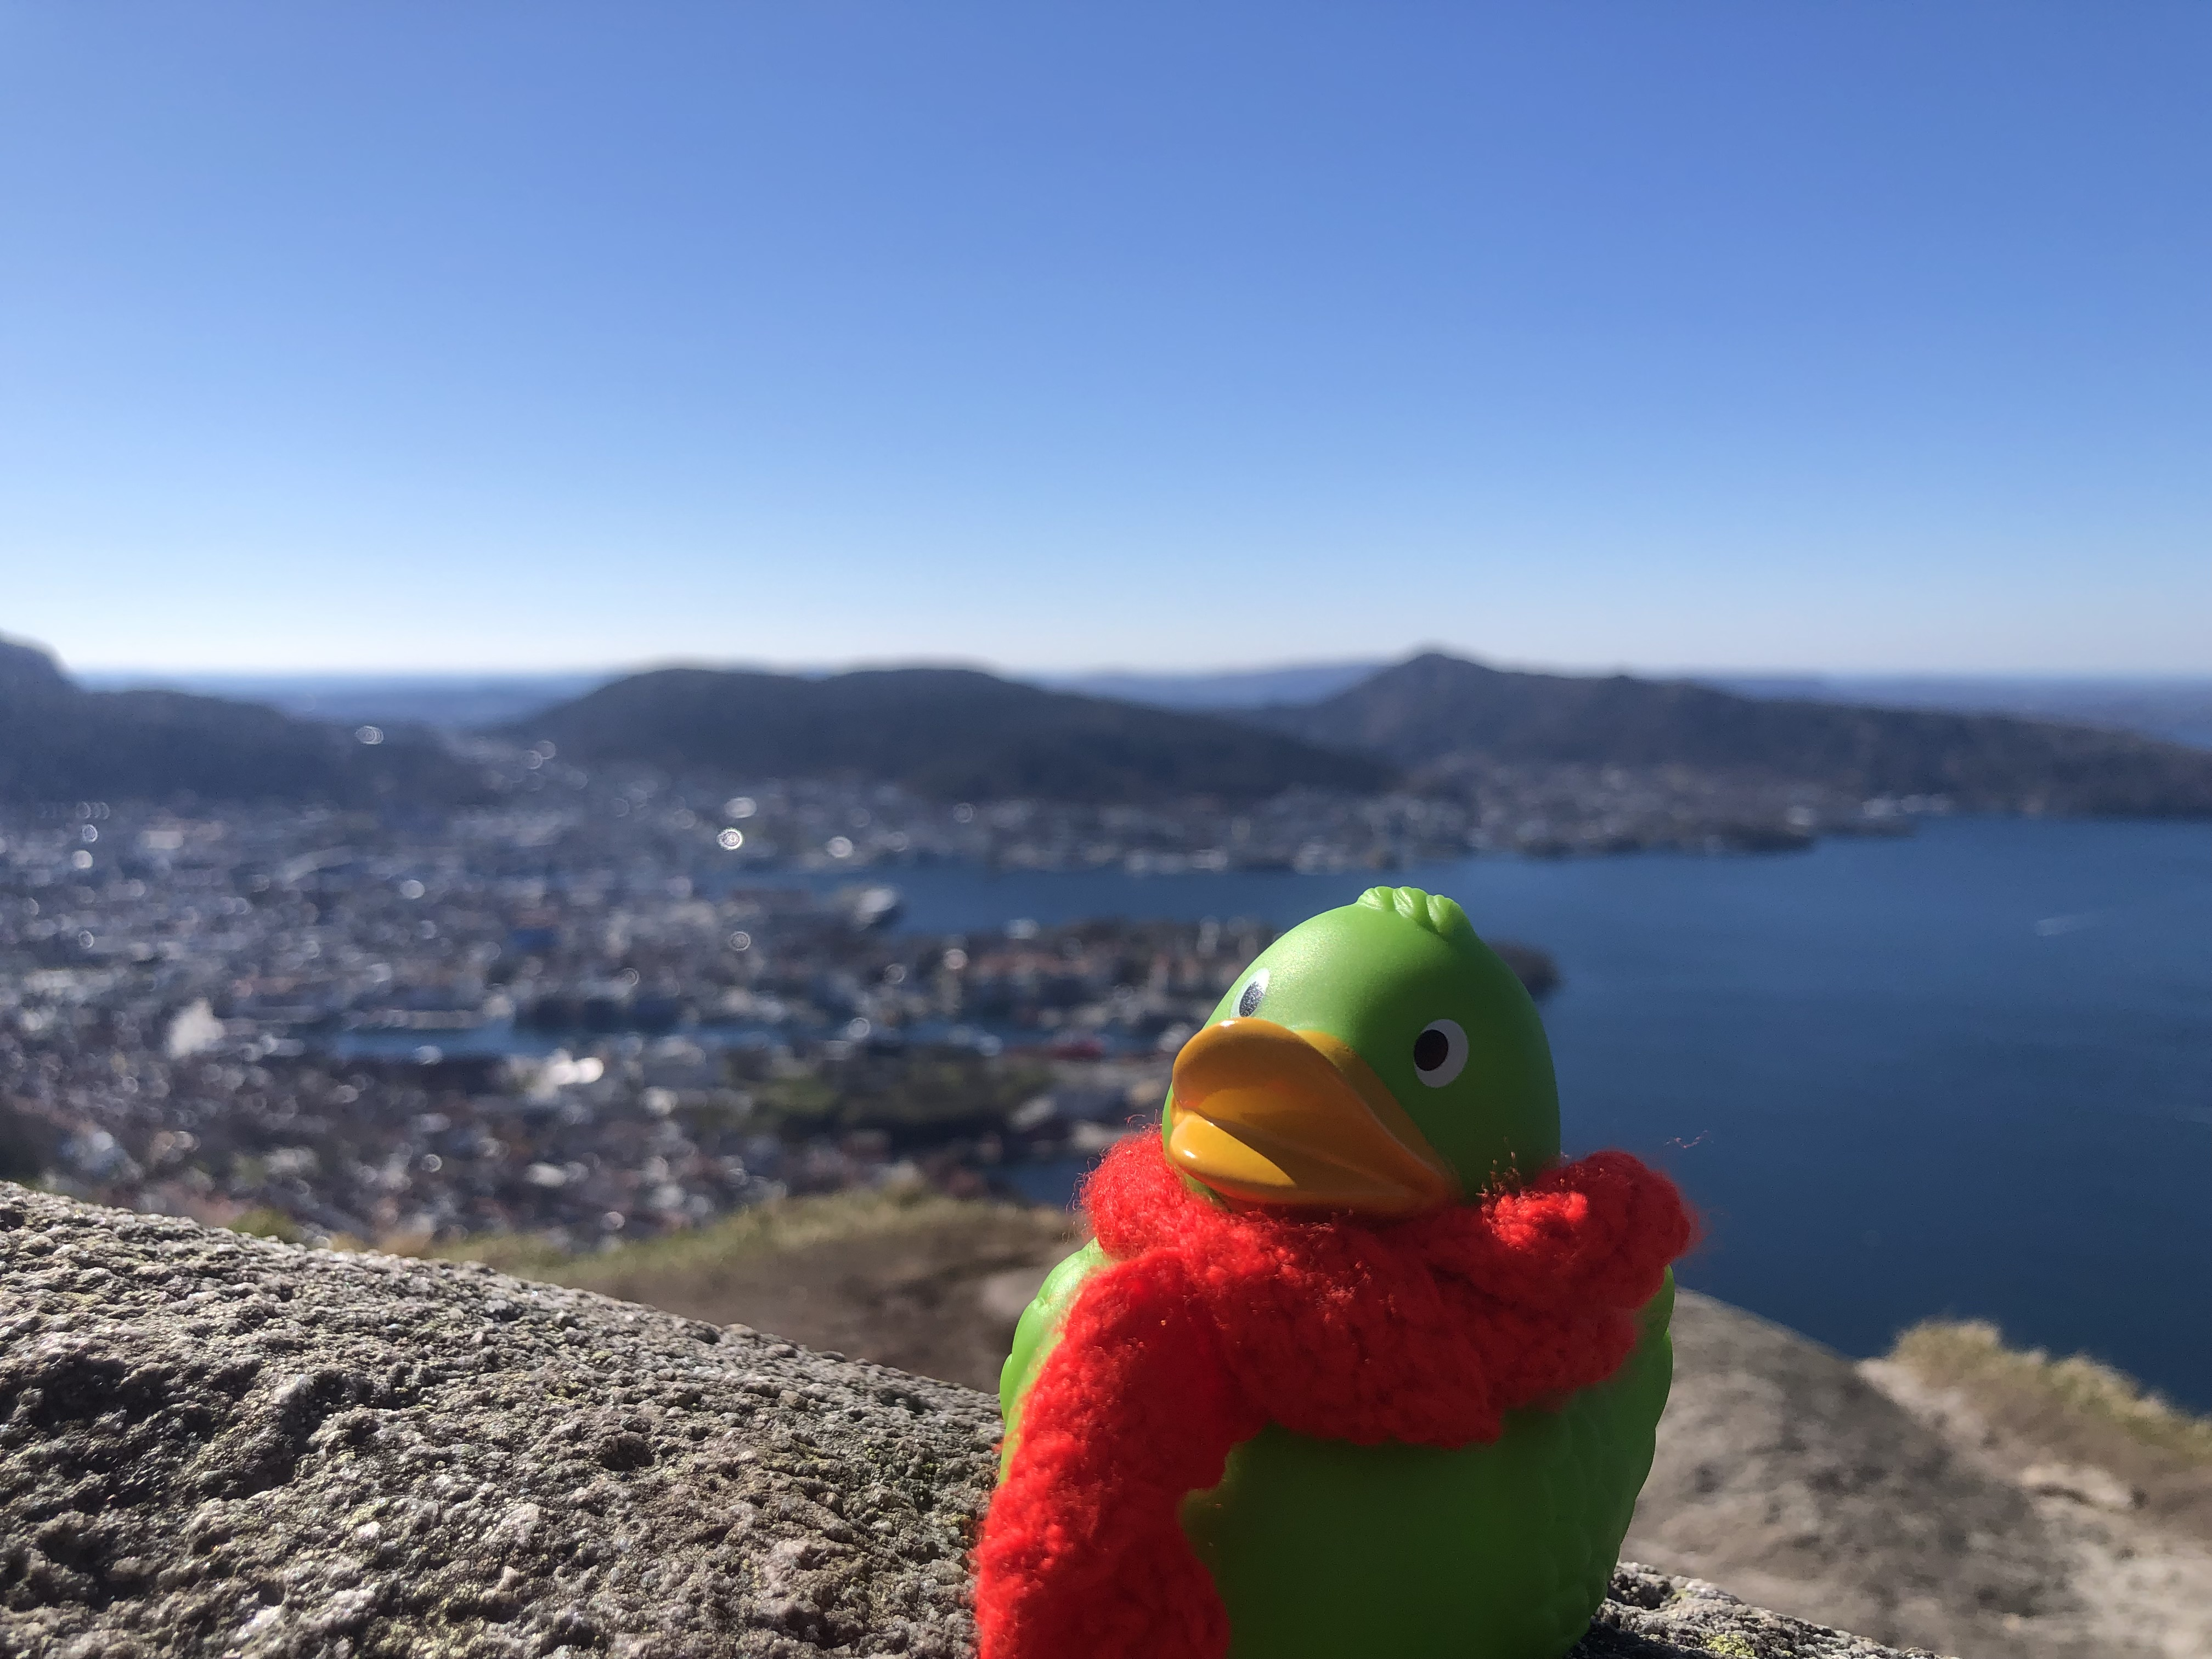
\includegraphics[height = 4.9cm]{images/guillaume1.jpg}
        \caption{Guillaume på Sandviksfjellet}
        \label{fig:guillaume1}
    \end{figure}
\end{frame}

\section{Relasjonsalgebra}
\subsection*{Operatorer}
\begin{frame}{Operatorer}
\begin{tabular}{l|l|l}
 Operator & Betydning & Eksempel\\\hline
 $\pi_{columns}(Tabell)$ & Projection (SELECT DISTINCT) & $\pi_{title, year}(Film)$\\
 $\sigma_{condition}(Tabell)$ & Condition (WHERE) & $\sigma_{year > 2015}(Film)$\\
 $A \times B$ & Cross join / Cartesian product & $Film \times Screening$\\
 $A \cap B$ & Intersection & $Film1 \cap Film2$ \\
 $A \cup B$ & Union & $Film1 \cup Film2$ \\
 $A \setminus B$ & Set difference &  $Film1 \setminus Film2$\\
 $A \bowtie_{condition} B$ & Inner Join & $A \bowtie_{film_{id}=film_{id}} B$\\
\end{tabular}
\end{frame}

\subsection*{Eksempler}
\begin{frame}[fragile]{Eksempel 1}
\begin{minted}{sql}
SELECT DISTINCT Country
FROM Film
WHERE year < 1950
\end{minted}
$\pi_{Country}\textcolor{blue}{(}\sigma_{year < 1950}\textcolor{red}{(}Film\textcolor{red}{)}\textcolor{blue}{)}$
\end{frame}

\begin{frame}[fragile]{Eksempel 2}
\begin{minted}{sql}
SELECT DISTINCT title, year
FROM Film, Director
WHERE Film.dir_id = Director.id
AND Film.year = 1992
\end{minted}
$\pi_{title, year}\textcolor{blue}{(}\sigma_{year = 1992}\textcolor{red}{(}Film\textcolor{red}{)} \bowtie_{Film.dir\_id=Director.id}\textcolor{red}{(}Director\textcolor{red}{)}\textcolor{blue}{)}$
\end{frame}

\begin{frame}[fragile]{Eksempel 3}
\begin{minted}{sql}
SELECT Country.name, capital, inhabitants
FROM Country, City
WHERE Country.capital = City.id
AND inhabitants < 500000
\end{minted}
$\pi_{Country.name, capital, inhabitants}\textcolor{blue}{(}\sigma_{inhabitants < 500000}\textcolor{green}{(}\textcolor{red}{(}Country\textcolor{red}{)}\bowtie_{Capital=City.id}\textcolor{red}{(}City\textcolor{red}{)}\textcolor{green}{)}\textcolor{blue}{)}$
\end{frame}

\subsection*{Spørretid}
\begin{frame}{Spørsmål?}
    \begin{figure}
        \centering
        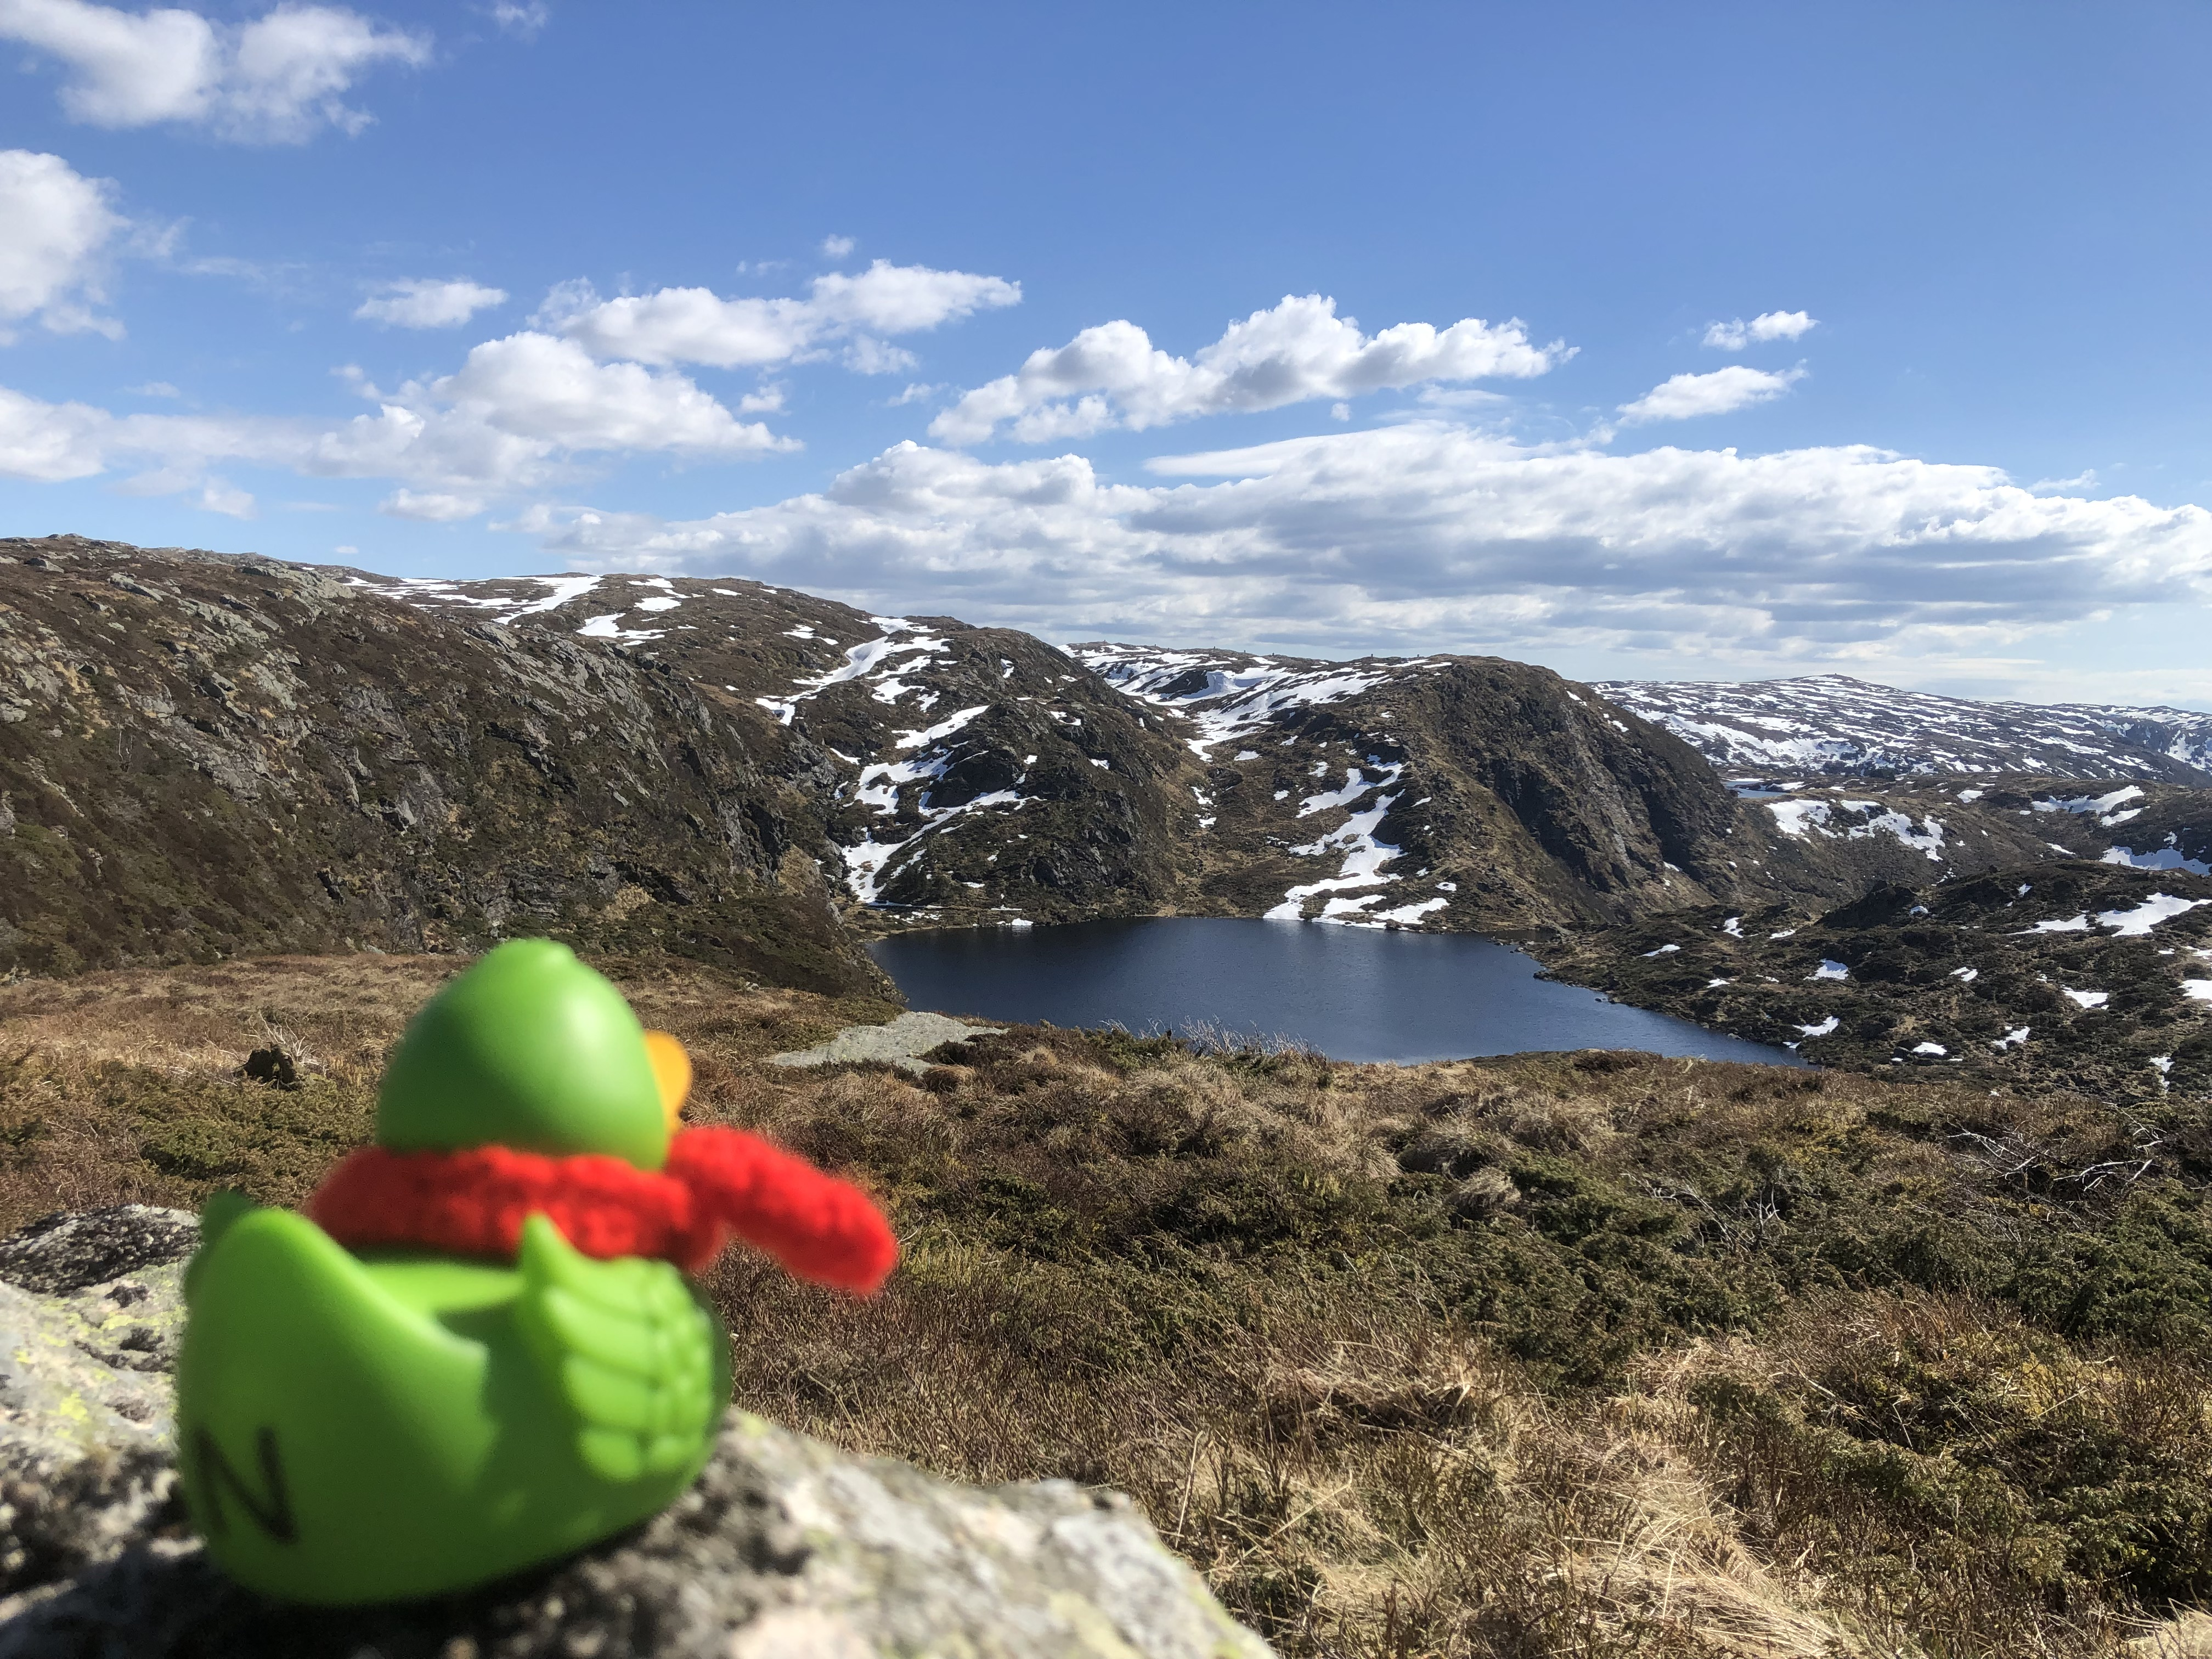
\includegraphics[height = 4.9cm]{images/guillaume4.jpg}
        \caption{Guillaume på Vidden}
        \label{fig:guillaume4}
    \end{figure}
\end{frame}

%=================================
%Fortsett her
%=================================

\section{ER-Diagrammer}
\begin{frame}{Entity-Relationship Diagrammer}
    \begin{itemize}
        \item Grafisk versjon av en database
        \item Identifikasjon av entiteter
        \item Identifikasjon av sammenheng mellom entiteter
    \end{itemize}
\end{frame}

\subsection*{Kardinalitet}
\begin{frame}{Kardinalitet}
\begin{columns}
    \begin{column}{0.48\textwidth}
\begin{tikzpicture}[every node/.style={font=\scriptsize}]
    \draw[mone-,thick] (0,0) -- node[above]{eksakt 1}node[below]{(1,1)} (5,0);
    \draw[mmany-,thick] (0,-1) -- node[above]{minst en}node[below]{(1,n)} (5,-1);
    \draw[oone-,thick] (0,-2) -- node[above]{opptil en}node[below]{(0,1)} (5,-2);
    \draw[omany-,thick] (0,-3) -- node[above]{ 0, 1 eller mange}node[below]{(0,n)} (5,-3);
    \end{tikzpicture}
 	\end{column}
    \begin{column}{0.48\textwidth}
\begin{tikzpicture}[every node/.style={font=\scriptsize}]
    \draw[mone-mone,thick] (0,0) -- node[above]{one-to-one}node[below]{} (5,0);
    \draw[mone-omany,thick] (0,-1) -- node[above]{one-to-many}node[below]{} (5,-1);
    \draw[omany-omany,thick] (0,-2) -- node[above]{many-to-many}node[below]{} (5,-2);
    \end{tikzpicture}
 	\end{column}
\end{columns}
    
\end{frame}

\begin{frame}{Eksempler}
    %\begin{itemize}
        %\item<1-1> Person - Fødselsby
        %\item<2-> Person (0,n) - (1,1) Fødselsby
        %\item<3-3> Kunde - Produkt
        %\item<4-> Kunde (0,n) - (0,n) Produkt
        %\item<5-5> Medarbeider - Prosjekt
        %\item<6-> Medarbeider (1,n) - (1,1) Prosjekt
        %\item<7-7> Land - Hovedstad
        %\item<8-> Land (1,1) - (1,1) Hovedstad
        %\item<9-9> Film - Regissør
        %\item<10-> Film (0,n) - (1,n) Regissør
        
    %\end{itemize}
\begin{tabular}{l|l|l}
    Tabell & Kardinalitet & Navn\\\hline
    Person - Fødselsby & (0,n) - (1,1) & one-to-many\\
    Kunde - Produkt & (0,n) - (0,n) & many-to-many\\
    Medarbeider - Prosjekt & (1,n) - (1,1) & one-to-many\\
    Land - Hovedstad & (1,1) - (1,1) & one-to-one\\
    Film - Regissør & (0,n) - (1,n) & many-to-many
    \end{tabular}
\end{frame}

\begin{frame}{}
    \begin{figure}
        \centering
        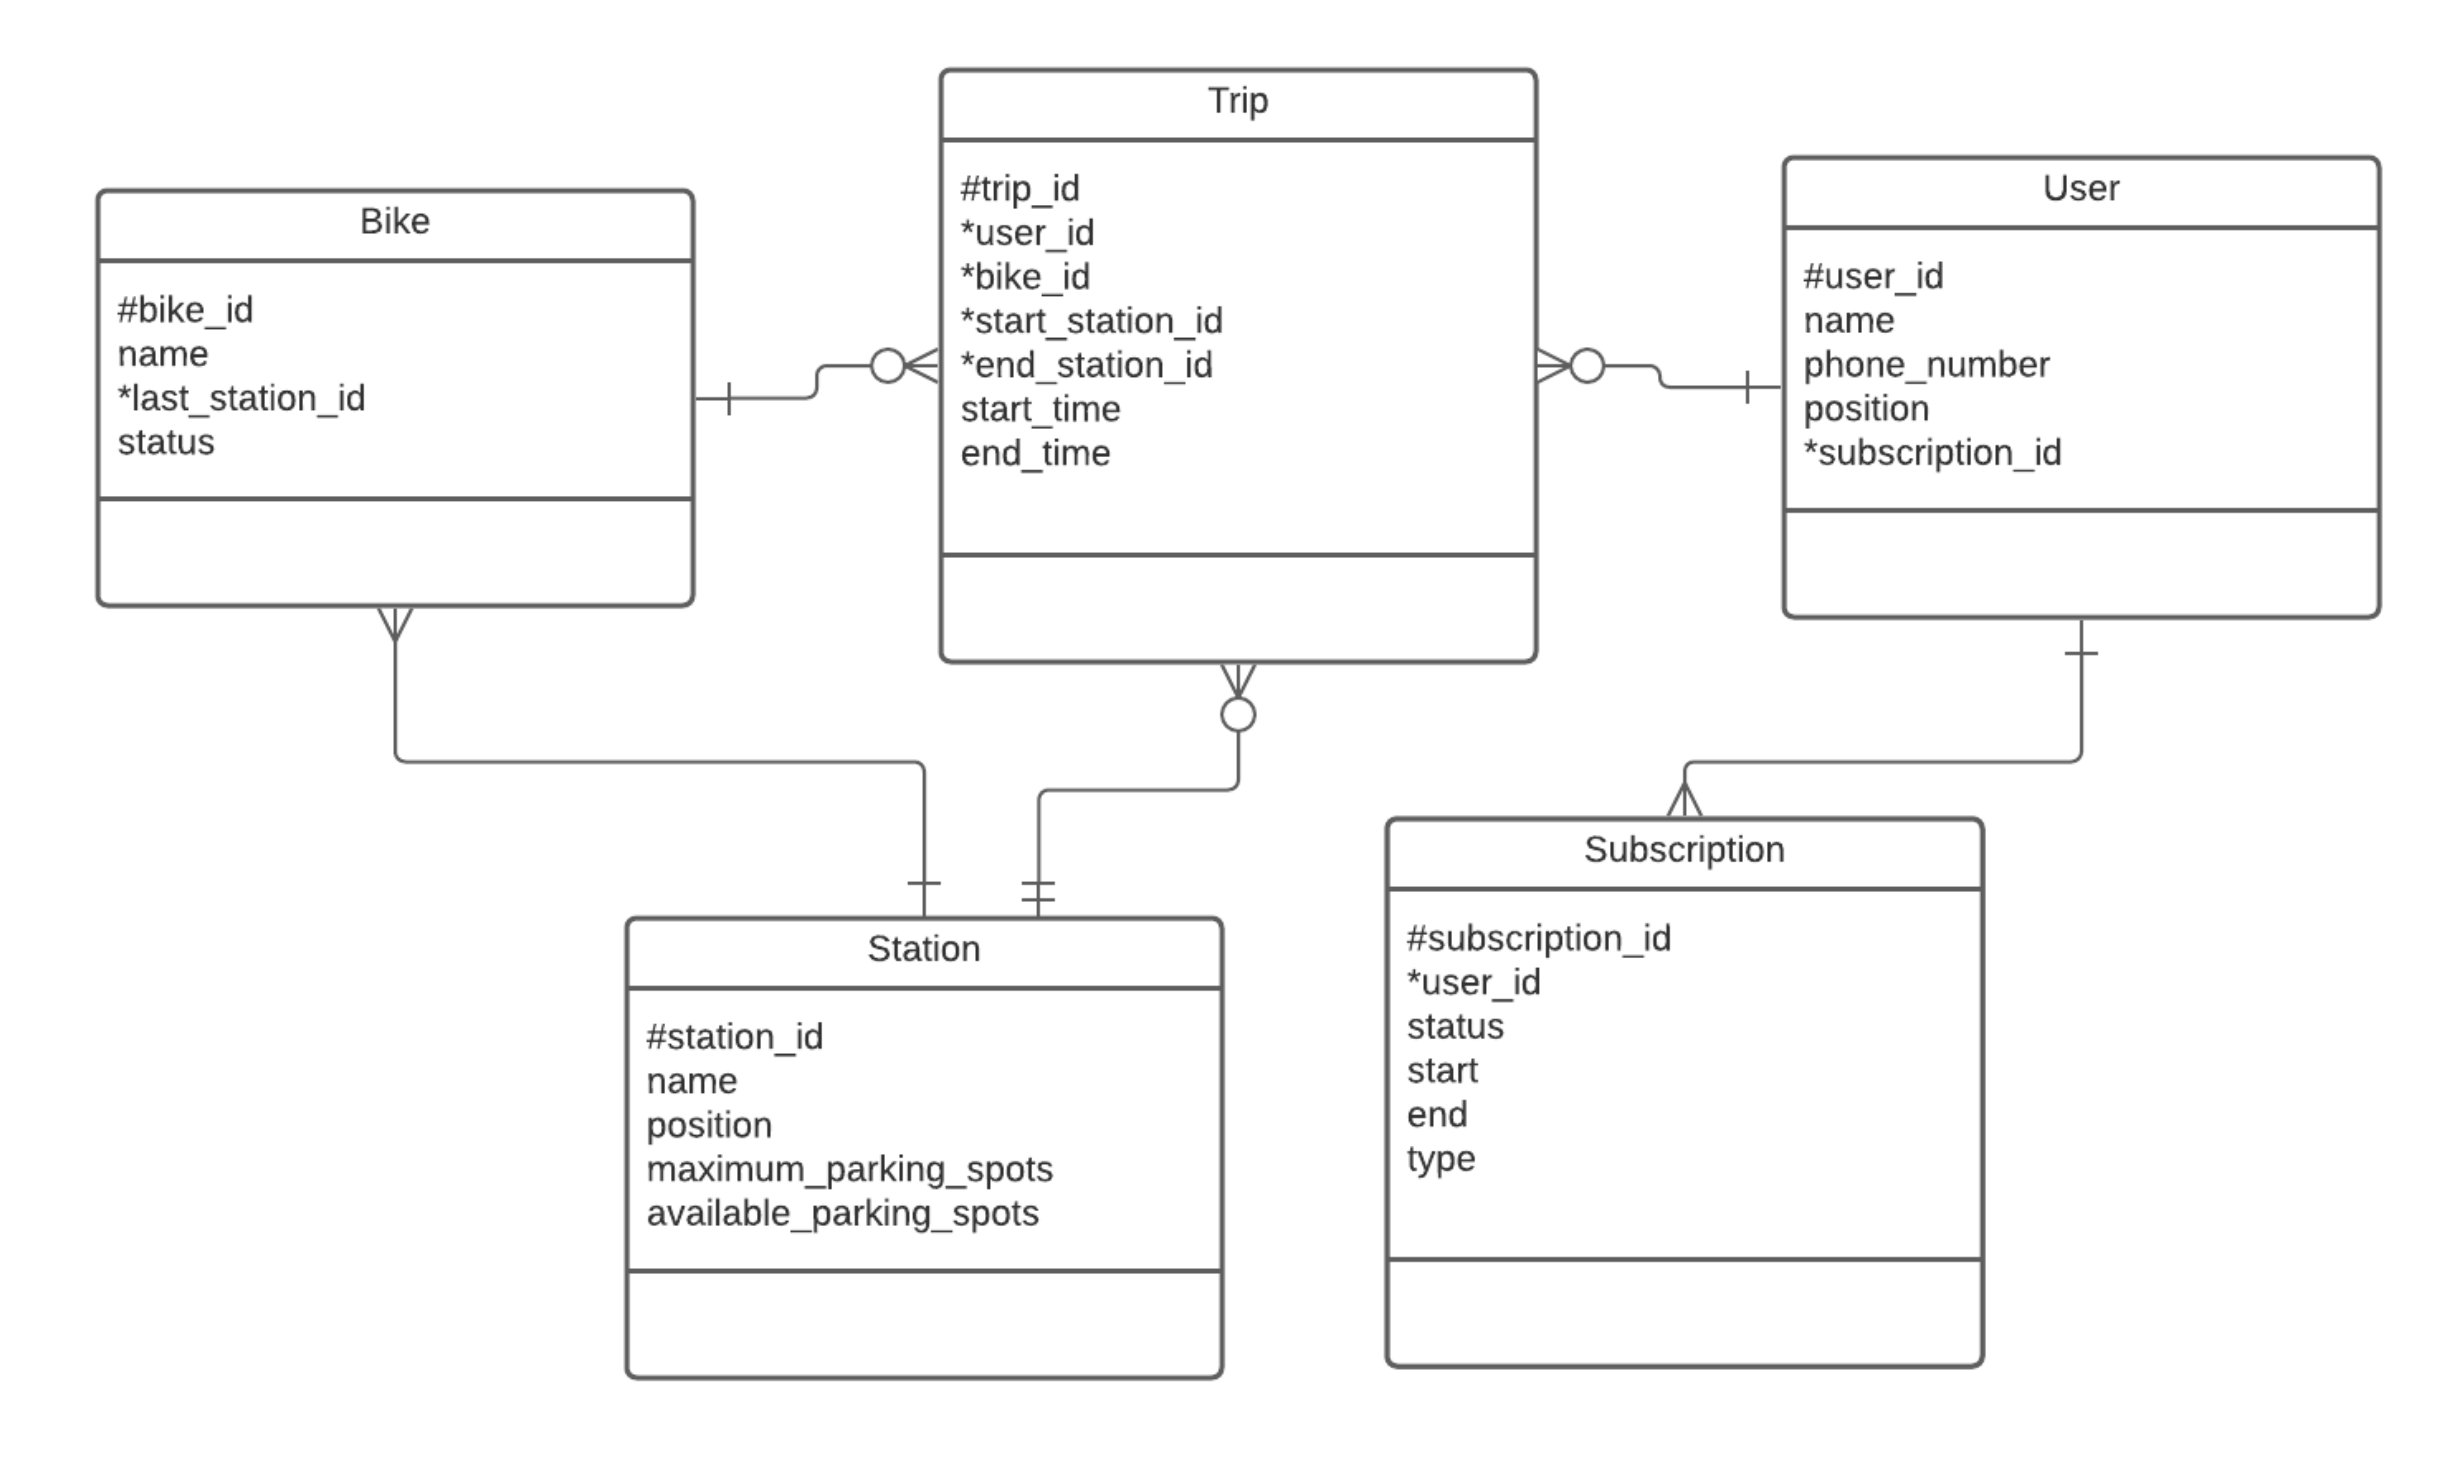
\includegraphics[height = 4.9cm]{images/erdiagram.png}
        \caption{Eksempel ER-diagram fra oblig 2}
        \label{fig:erdiagram}
    \end{figure}
\end{frame}

\subsection*{Spørretid}
\begin{frame}{Spørsmål?}
    \begin{figure}
        \centering
        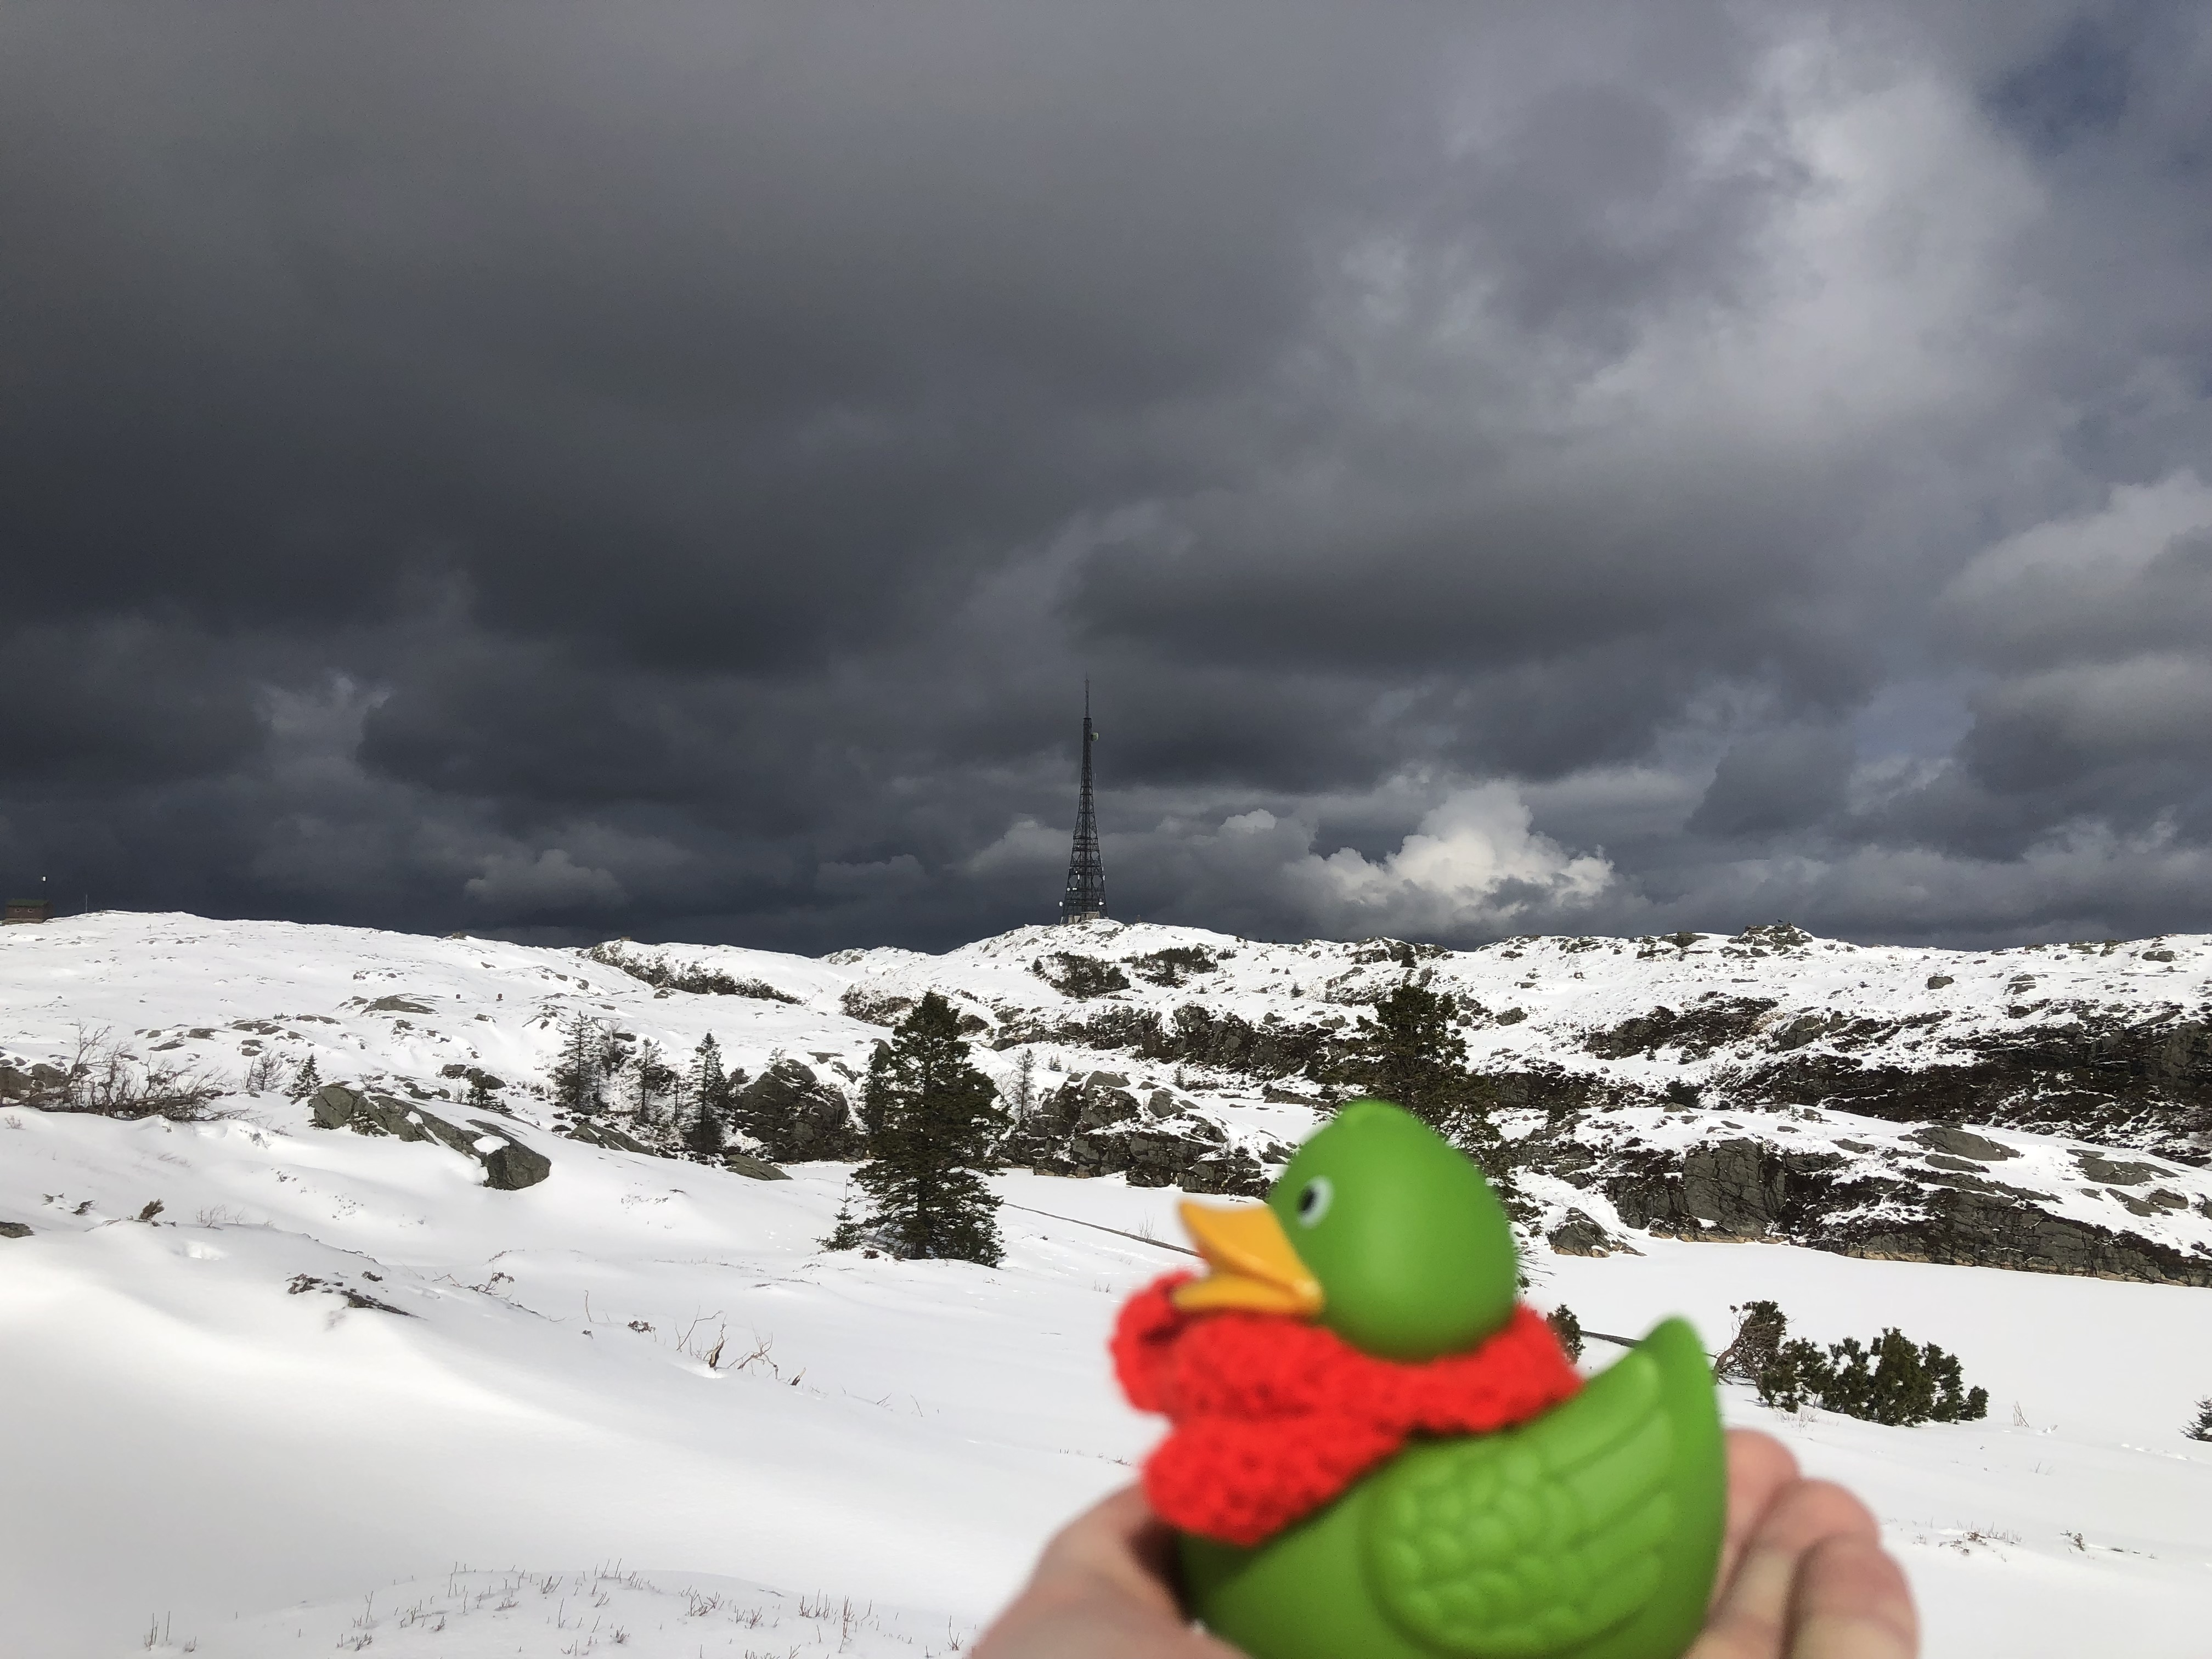
\includegraphics[height = 4.9cm]{images/guillaume6.jpg}
        \caption{Guillaume på Blåmanen}
        \label{fig:guillaume6}
    \end{figure}
\end{frame}

%=================================

\section{Normalisasjon}
\subsection*{Hvorfor gjør man normalisasjon?}
\begin{frame}{Hvorfor normalisasjon?}
\begin{itemize}
    \item Unngå redundante informasjoner
    \item Bedre å oppdatere informasjoner hvis de bare finnes en gang
    \item Lettere å bruke en stor database
    \item Visualisering av en database
\end{itemize}
\end{frame}

\subsection*{Viktige begrep}
\begin{frame}{Begrep}
\begin{itemize}
    \item \textbf{Entitet: }En tabell i databasen
    \item \textbf{Attributt: }En spalte i en tabell
    \item \textbf{Nøkkel: }En spalte som bestemmer en/noen flere spalter
    \item \textbf{Supernøkkel: }En nøkkel som bestemmer alle andre spaltene
    \item \textbf{Kandidatnøkkel: }En minimal supernøkkel
\end{itemize}
\end{frame}

\begin{frame}{Functional Dependencies}
\begin{itemize}
    \item En eller flere spalter bestemmer verdier av andre spalter
    \item $A \rightarrow B$ (A bestemmer B)
    \item $A,B \rightarrow C, D, E$ (A og B bestemmer C, D og E)
    \item PersonNr $\rightarrow$ Navn (det samme nummer er det samme person)
    \item ZipCode $\rightarrow$ City (den samme postkoden er den samme byen)
\end{itemize}
\end{frame}

\subsection*{Anomalier}
\begin{frame}{Eksempel}
%\begin{center}
\begin{tabular}{l|l|l|l|l}
 StudentNr & Name & Address & KursNr & KursName \\\hline
 580 & Ola NordmaNN & 5075 Bergen Fv 14 & INF237 & Algorithm Engineering\\
 580 & Ola NordmaNN & 5075 Bergen Fv 14 & INF273 & Meta Heuristikker\\
 580 & Ola NordmaNN & 5075 Bergen Fv 14 & INF227 & Logik\\
 256 & Max MustermaNN & 5055 Bergen Lv 85 & INF237 & Algorithm Engineering\\
\end{tabular}
\\[5mm]
Hva er problemet her?\\
Informasjoner blir lagret dobbelt.\\
Hvis kursnavn eller studentadressen endrer seg, må den endres flere ganger.
%\end{center}
\end{frame}

\begin{frame}{Anomalier}
\begin{itemize}
    \item Insertion Anomaly: Den samme informasjonen blir lagt inn med andre verdier
    \item Update Anomaly: Dobbel informasjon blir ikke oppdatert overalt
    \item Deletion Anomaly: Data forsvinner fordi den ikke finnes i en egen tabell
\end{itemize}
\medskip
Eksempler:
\begin{itemize}
    \item Insertion Anomaly: Studenten tar et kurs til, men har nå en annen adresse 
    \item Update Anomaly: Kursnavnet blir oppdatert, men ikke for alle studenter
    \item Deletion Anomaly: En student melder seg ut av alle kurser, så forsvinner han i hele databasen
\end{itemize}
\end{frame}

\begin{frame}{Hvordan løser man problemene?}
\begin{tabular}{l|l|l}
 StudentNr & Name & Address\\\hline
 580 & Ola NordmaNN & 5075 Bergen Fv 14\\
 256 & Max MustermaNN & 5055 Bergen Lv 85\\
\end{tabular}
\vfill
\begin{tabular}{l|l}
KursNr & KursName \\\hline
INF237 & Algorithm Engineering\\
INF273 & Meta Heuristikker\\
INF227 & Logikk\\
\end{tabular}
\hfill
\begin{tabular}{l|l}
 StudentNr & KursNr\\\hline
 580 & INF237\\
 580 & INF273\\
 580 & INF227\\
 256 & INF237\\
\end{tabular}
\end{frame}

\subsection*{Normalformer}
\begin{frame}{1. Normalform (1NF)}
    \begin{block}{1. Normalform}
    Hvert attributt (spalte) må være atomar, den kan ikke har flere verdier (lister etc. er forbud).
    \end{block}
    \vfill
    \begin{tabular}{l|l}
     StudentNr & KursNr\\\hline
     580 & [INF237, INF273, INF227]\\
     256 & INF237\\
     \end{tabular}
     \hfill
     $\rightarrow$
     \hfill
     \begin{tabular}{l|l}
     StudentNr & KursNr\\\hline
     580 & INF237\\
     580 & INF273\\
     580 & INF227\\
     256 & INF237\\
    \end{tabular}
\end{frame}

\begin{frame}{2. Normalform (2NF)}
    \begin{block}{2. Normalform}
    Alle ikke-nøkkel-attributter er fullstendig funksjonell avhengig av en primærnøkkel.\\
    En ikke primær-attributt kan ikke være avhengig av bare en del av nøkkelen.
    \end{block}
    \vfill
    \only<1>{\begin{tabular}{l|l|l}
     StudentNr & KursNr & StudentNavn\\\hline
     580 & INF237 & Ola\\
     580 & INF273 & Ola\\
     580 & INF227 & Ola\\
     256 & INF237 & Max\\
     \end{tabular}
     }
     \only<2>{
     \begin{tabular}{l|l}
     StudentNr & KursNr\\\hline
     580 & INF237\\
     580 & INF273\\
     580 & INF227\\
     256 & INF237\\
    \end{tabular}
    \hfill
    \begin{tabular}{l|l}
     StudentNr & StudentNavn\\\hline
     580 & Ola\\
     580 & Ola\\
     580 & Ola\\
     256 & Max\\
    \end{tabular}
    }
\end{frame}

\begin{frame}{3. Normalform (3NF)}
\begin{block}{3. Normalform}
    Det finnes ingen transitive avhengigheter.\\
    Det finnes ikke tre attributter A, B, C der $A \rightarrow B$ og $B \rightarrow C$ gjelder.
    \end{block}
    \vfill
    \only<1>{\begin{tabular}{l|l|l}
     Universitetet & By & Land\\\hline
     UiB & Bergen & Norge\\
     HUB & Berlin & Tyskland\\
     NTNU & Trondhjem & Norge\\
     \end{tabular}
     }
     \only<2>{
     \begin{tabular}{l|l}
     Universitetet & By\\\hline
     UiB & Bergen\\
     HUB & Berlin\\
     NTNU & Trondhjem\\
    \end{tabular}
    \hfill
    \begin{tabular}{l|l}
     By & Land\\\hline
     Bergen & Norge\\
     Berlin & Tyskland\\
     Trondhjem & Norge\\
    \end{tabular}
    }
\end{frame}

\begin{frame}{Boyce–Codd Normalform (BCNF)}
\begin{block}{Boyce-Codd Normalform ($3 \frac{1}{2}$NF)}
    Det finnes ikke to overlappende kandidatnøkler. Skjer nesten aldri.
    \end{block}
    \vfill
    $Tabell(A, B, C, D)$\\
    $A,B\rightarrow C,D; $ $C\rightarrow B$\medskip
    
    \pause
    Løsning: Split opp tabellen for å fjerne syklisk avhengig:\\
    $Tabell1(A, C, D)$, $Tabell2(C, B)$\\
    $A\rightarrow C,D; $ $C\rightarrow B$\medskip
\end{frame}

\subsection*{Spørretid}
\begin{frame}{Spørsmål?}
    \begin{figure}
        \centering
        \includegraphics[height = 4.9cm]{images/guillaume9.jpg}
        \caption{Guillaume foran Tvindefossen}
        \label{fig:guillaume9}
    \end{figure}
\end{frame}

%=================================

\section{Indekser}
\subsection*{Hvorfor indekser?}
\begin{frame}{Indekser}
    \begin{itemize}
        \item Rows er ikke sortert
        \item $\rightarrow$ finne informasjoner med WHERE tar tid
        \item Indekser er ekstrastrukturer som forenkler søking i tabellen
        \item Kan være en eller flere spalter
        \item Indekser funker som ordbok/lookup table
        \item Ulempe: De tar plass, må oppdateres
        \item To typer indekser:
            \begin{itemize}
                \item B-trær
                \item Hashing
            \end{itemize}
    \end{itemize}
\end{frame}

\subsection*{B-trær}
\begin{frame}{B-trær}
    \begin{itemize}
        \item innhold
    \end{itemize}
\end{frame}

\subsection*{Hashing}
\begin{frame}{Hashing}
    \begin{itemize}
        \item innhold
    \end{itemize}
\end{frame}

\subsection*{Eksempel}
\begin{frame}{Hvilke indeks skulle man ha?}
    \begin{itemize}
        \item innhold
    \end{itemize}
\end{frame}

\subsection*{Spørretid}
\begin{frame}{Spørsmål?}
    \begin{figure}
        \centering
        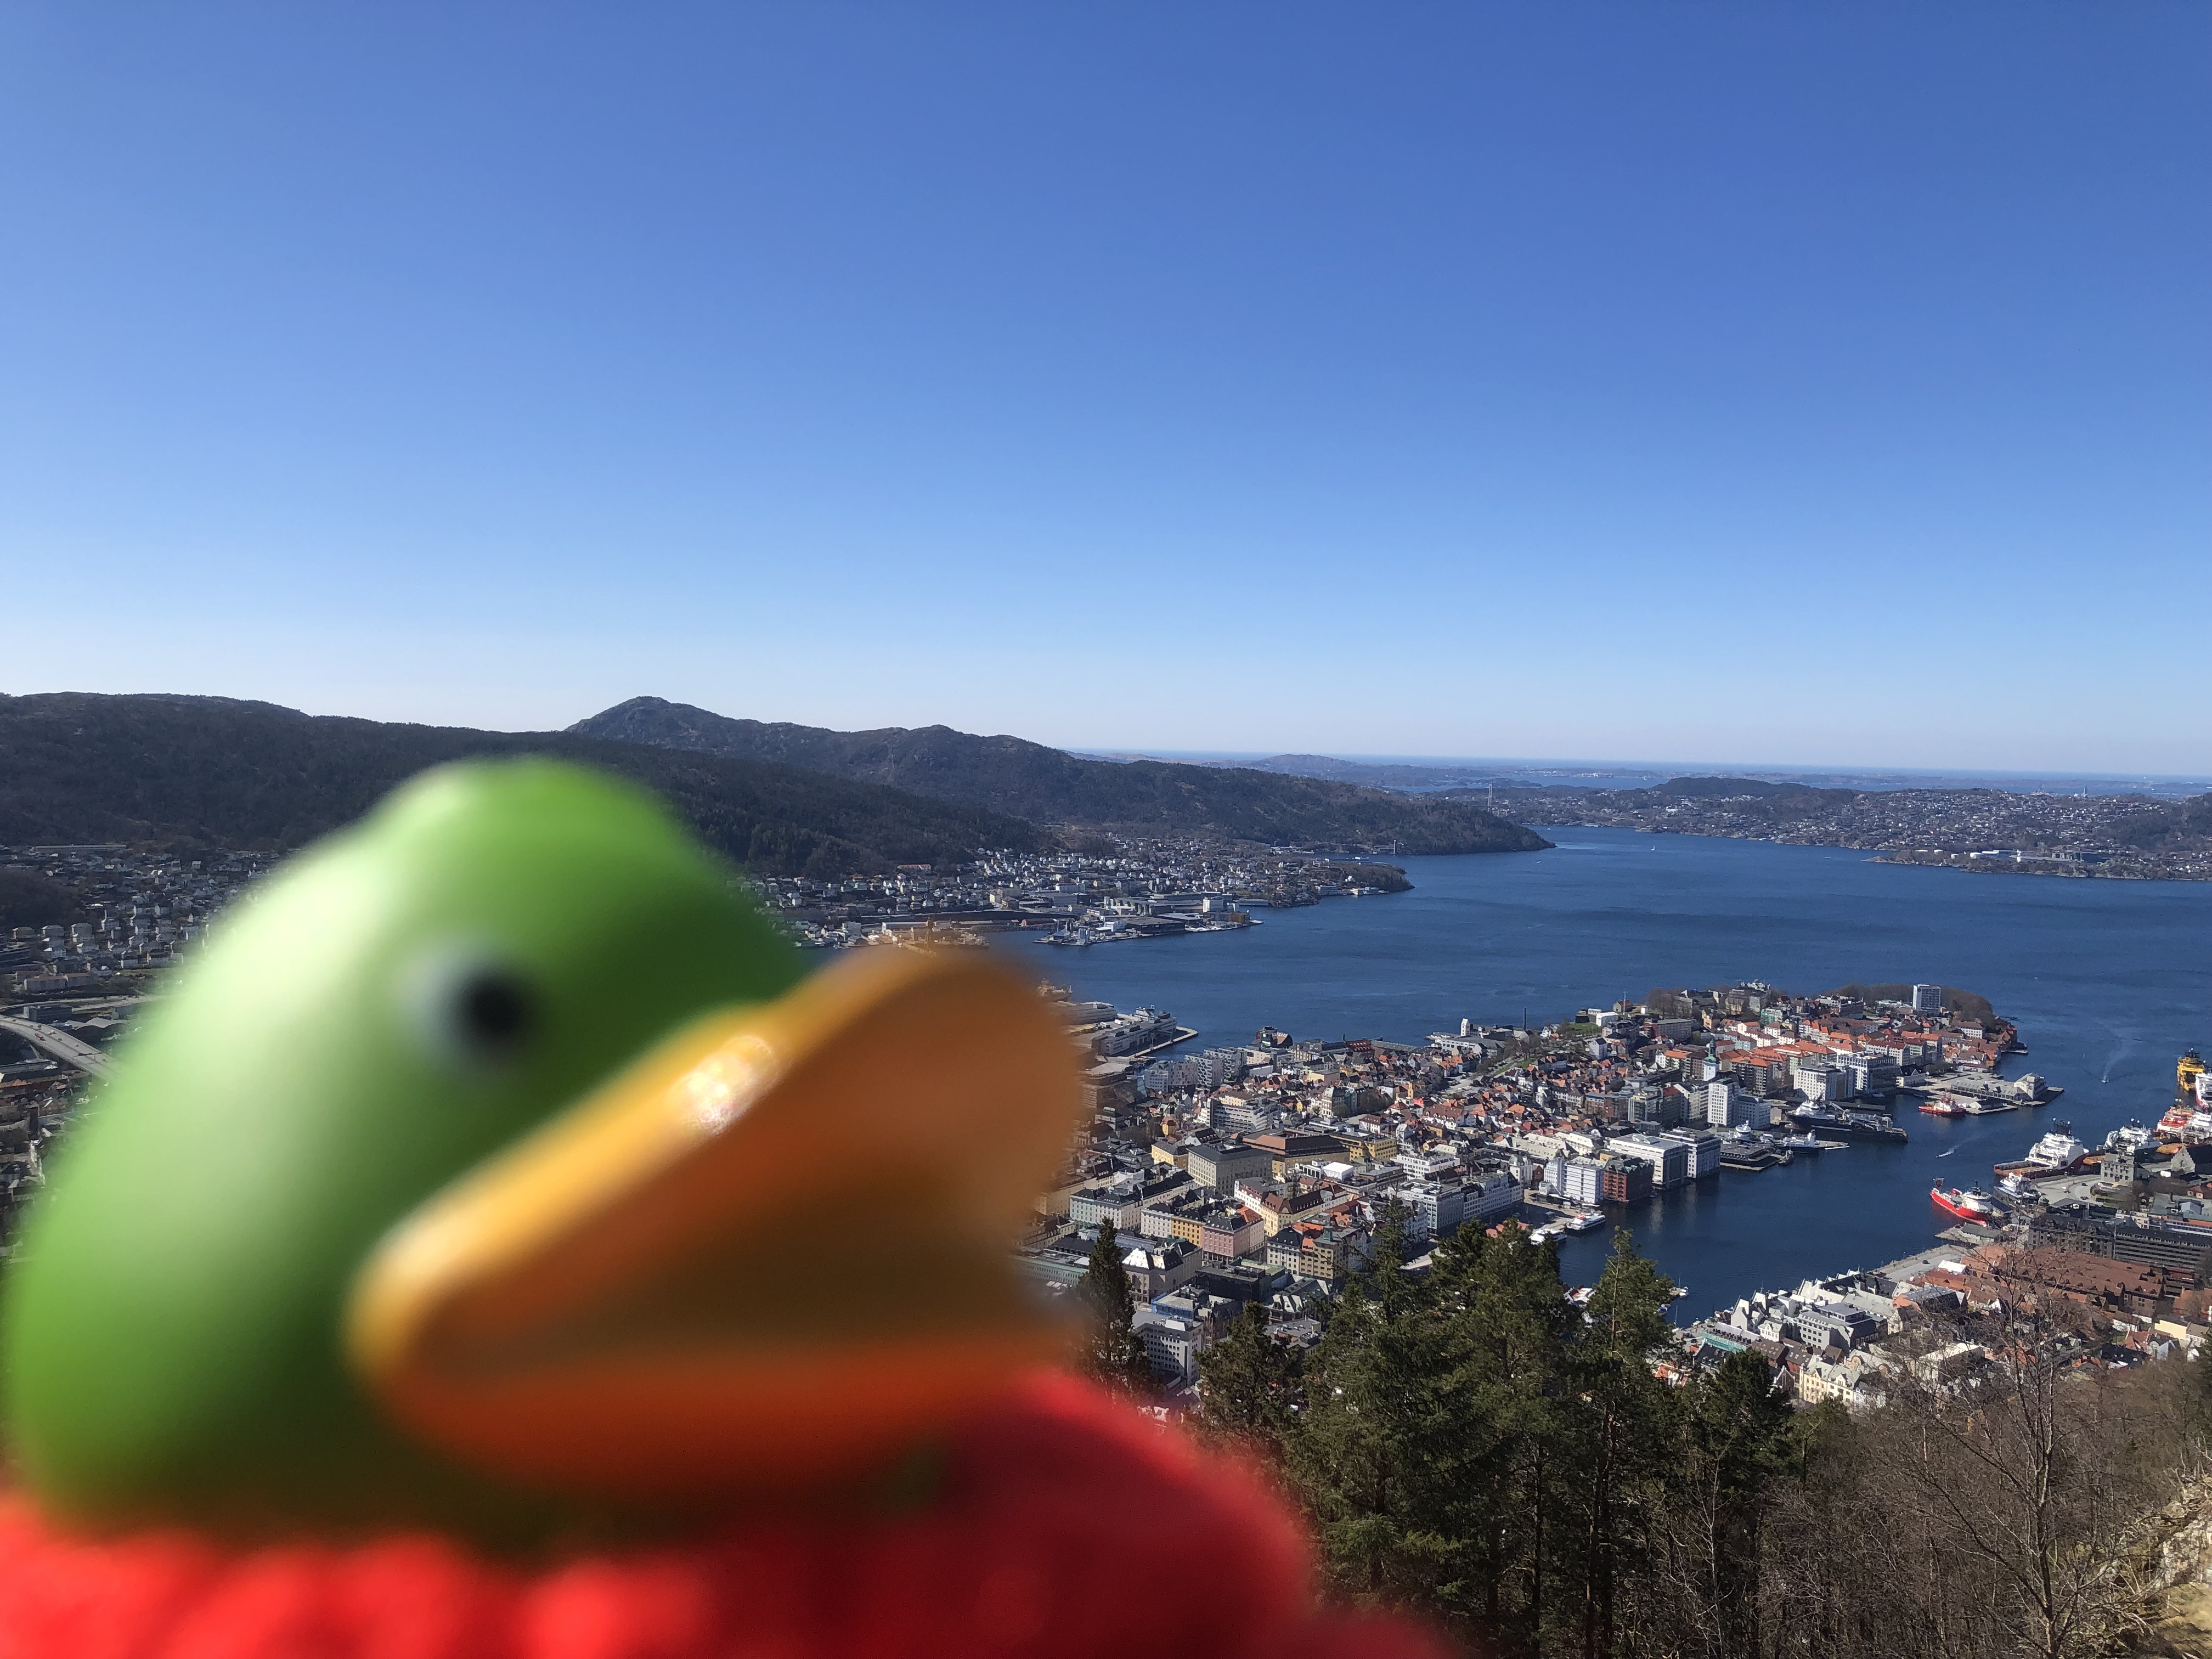
\includegraphics[height = 4.9cm]{images/guillaume10.jpg}
        \caption{Guillaume på Fløyen}
        \label{fig:guillaume10}
    \end{figure}
\end{frame}

%=================================

\section{Transaksjoner}
\begin{frame}{Hvorfor Transactions?}
    \begin{itemize}
        \item Sammenfatte flere kommandoer til en transaksjon
        \item Passe på at alt eller ingenting blir utført
        \item Passe på at flere kommandoer ikke blandes meg hverandre
    \end{itemize}
\end{frame}

\begin{frame}{ACID Prinsipper}
    \begin{itemize}
        \item Atomicity: Alt eller ingenting blir utført.
        \item Consistency: Databasen går fra en gyldig til en gyldig status.
        \item Isolation: Parallele transaksjoner ser ikke hverandre.
        \item Durability: Resultater av en transaksjon blir ikke overskrevet av den neste transaksjonen.
    \end{itemize}
\end{frame}

\subsection*{Ting som kan gå galt}
\begin{frame}{}
    \begin{block}{Lost Update}
    To transaksjoner jobber på samme tall på samme tidspunkt og den ene overskrever den andres verdien.
    \end{block}
    \begin{itemize}
        \item Vi får samtidig 1.000 kr fra bestemoren (A) og betaler 100kr til hvem som helst (B)
        \item A leser verdien på kontoen (5000kr)
        \item B leser verdien på kontoen (5000kr)
        \item A legger til 1.000kr og skriver verdien tilbake til databasen (6000kr)
        \item B fjerner 100kr og skriver verdien tilbake til databasen (4900kr)
        \item B har overskrevet resultatet til A
    \end{itemize}
    
\end{frame}

\begin{frame}{}
    \begin{block}{Aborted Update}
    En kommando ikke blir tilbakegjort etter rollback.
    \end{block}
    \begin{itemize}
        \item A sender 100kr til B
        \item Banken fjerner 100kr fra kontoen til A
        \item Det skjer en feil når man gir 100kr til B
        \item Nå har A tapt 100kr, men B ikke fått 100kr
        \item Databasen må nå rette kontoen til A
    \end{itemize}
\end{frame}

\begin{frame}{}
    \begin{block}{Inconsistent Analysis}
    En kommando baserer seg på både gamle data og nye data samtidig.
    \end{block}
    \begin{itemize}
        \item Vi skal legge til en film og en screening i databasen
        \item I tillegg skal vi få en joined tabell med alle filmer og screenings til sammen
        \item Hvis man legger til film, kjører JOIN kommandoen og etterpå legger til screening, har vi \textit{inconsistent analysis}
        \item Kommandoen baserer informasjoner på gamle verdier (screening tabell) og nye verdier (film database) samtidig
        \item Enten gjør alle INSERT på begynnelsen eller på slutten
    \end{itemize}
\end{frame}

\subsection*{SQL Transaksjoner}
\begin{frame}[fragile]{Transaksjoner i SQL}
\begin{minted}{sql}
START TRANSACTION;      -- her starter transaksjonen
UPDATE bankaccount      -- ta 20kr fra en bankkonto 
SET money = money - 20  -- dette er ikke korrekt syntaks
WHERE customer = 42;
UPDATE bankaccount      -- gi de 20kr til en annen bankkonto
SET money = money + 20
WHERE customer = 20;
COMMIT;                 -- commit hvis alt gikk fint, ellers rollback
-- ROLLBACK
\end{minted}
\end{frame}

\subsection*{Begrep}
\begin{frame}
\begin{itemize}
    \item Serialisability: To transaksjoner er serialisable dersom det finnes en rekkefølge de kan utføres uten at de ignorerer ACID-prinsippene
    \item Write lock: Variabel kan ikke endres, men verdien kan leses 
    \item Read lock: Variabel kan verken leses eller endres
    \item Two phase locking: Blokker alle variabler samtidig, frigir dem samtidig
\end{itemize}
\end{frame}

\subsection*{Waiting graph}
\begin{frame}{Finne rekkefølge for SQL kommandoer}
\begin{itemize}
    \item Lag rettet graf med transaksjoner som noder
    \item A venter til B: $A \rightarrow B$ (retningen antiintuitiv)
    \item Finn en rekkefølge å gå gjennom nodene
    \item Hvis graf har sykler finnes ikke en sånn rekkefølge
    \item Fjern de eldste transaksjonene inntil ingen sykler er igjen
\end{itemize}
\end{frame}

\begin{frame}{Eksempel}
\begin{columns}
    \begin{column}{0.48\textwidth}
\begin{tikzpicture}[
    node distance=1.45cm, thick,
    main node/.style={circle, draw, font=\sffamily\bfseries}
]
    \node<-4>[main node] (1)                    {1};
    \node[main node,onslide=<8>{fill=black!60!green}] (3) [below left  of=1] {3};
    \node[main node,onslide=<7->{fill=black!60!green}] (4) [below right of=1] {4};
    \node[main node,onslide=<3->{fill=black!60!green}] (2) [above right of=4] {2};
    \node[main node,onslide=<4->{fill=black!60!green}] (6) [below right of=4] {6}; % <-4> forces an additional overlay in which node 2 disappears

    \path<1>[->] (1) edge (2)
        (4) edge (2)
        (6) edge (2);
    \path<-4>[->] (1) edge (3)
        (4) edge (1);
    \path<-5>[->] (3) edge (4);
\end{tikzpicture}
 \end{column}
    \begin{column}{0.48\textwidth}
\begin{itemize}
    \item<1-> Graf med fem noder 
    \item<2-> Transaksjon 2 venter på ingenting
    \item<3-> Marker transaksjon 2 som utført
    \item<4-> Marker transaksjon 6 som utført
    \item<5-> Funnet syklus, fjern eldeste transaksjon 1
    \item<6-> Transaksjon 4 venter på ingenting
    \item<7-> Marker transaksjon 4 som utført
    \item<8-> Marker transaksjon 3 som utført
\end{itemize}
 \end{column}
\end{columns}
\end{frame}

\subsection*{Spørretid}
\begin{frame}{Spørsmål?}
    \begin{figure}
        \centering
        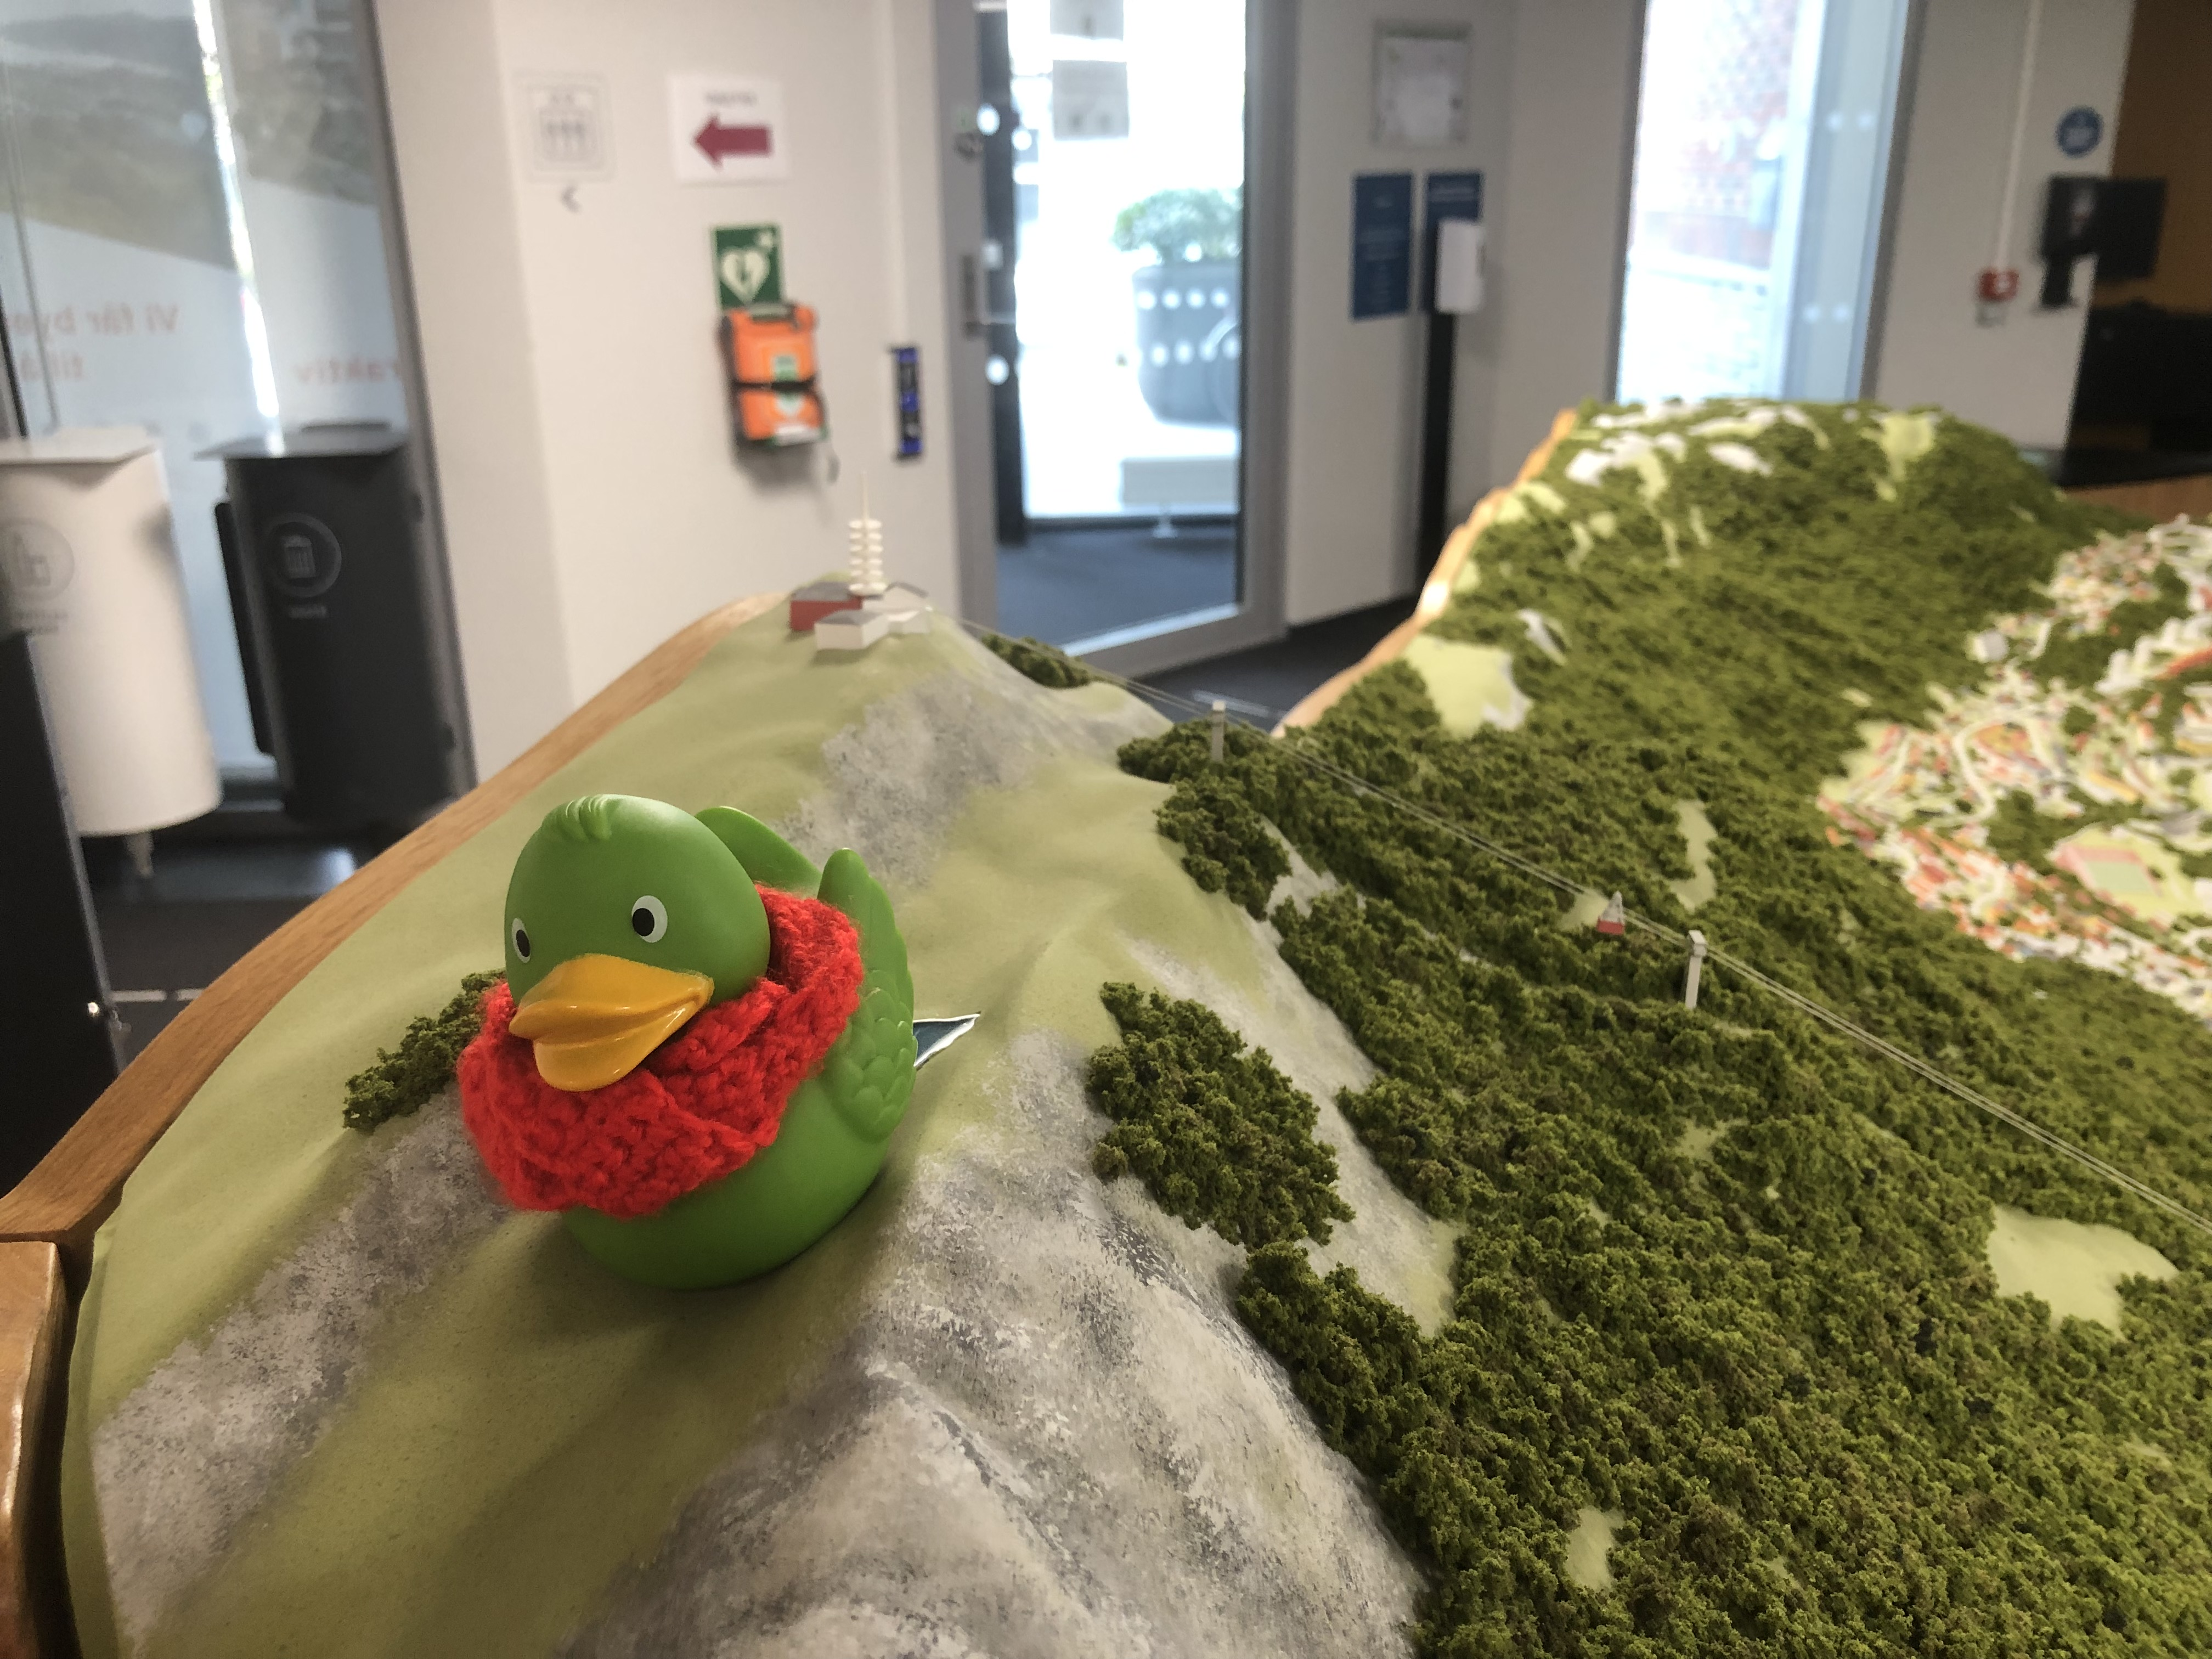
\includegraphics[height = 4.9cm]{images/guillaume11.jpg}
        \caption{Guillaume på Ulriken}
        \label{fig:guillaume11}
    \end{figure}
\end{frame}

%=================================

\section{Alt mulig}
\begin{frame}{Andre teamer}
\begin{itemize}
    \item Databaseadministrasjon
    \item Webapplikasjoner (php, tragisk)
    \item NoSQL, XML, JSON
    \item Noen småteamer og informasjoner fra temaene i kræsjkurset
    \item Guest Lectures
\end{itemize}
\end{frame}

\subsection*{Spørretid}
\begin{frame}{Spørsmål?}
    \begin{figure}
        \centering
        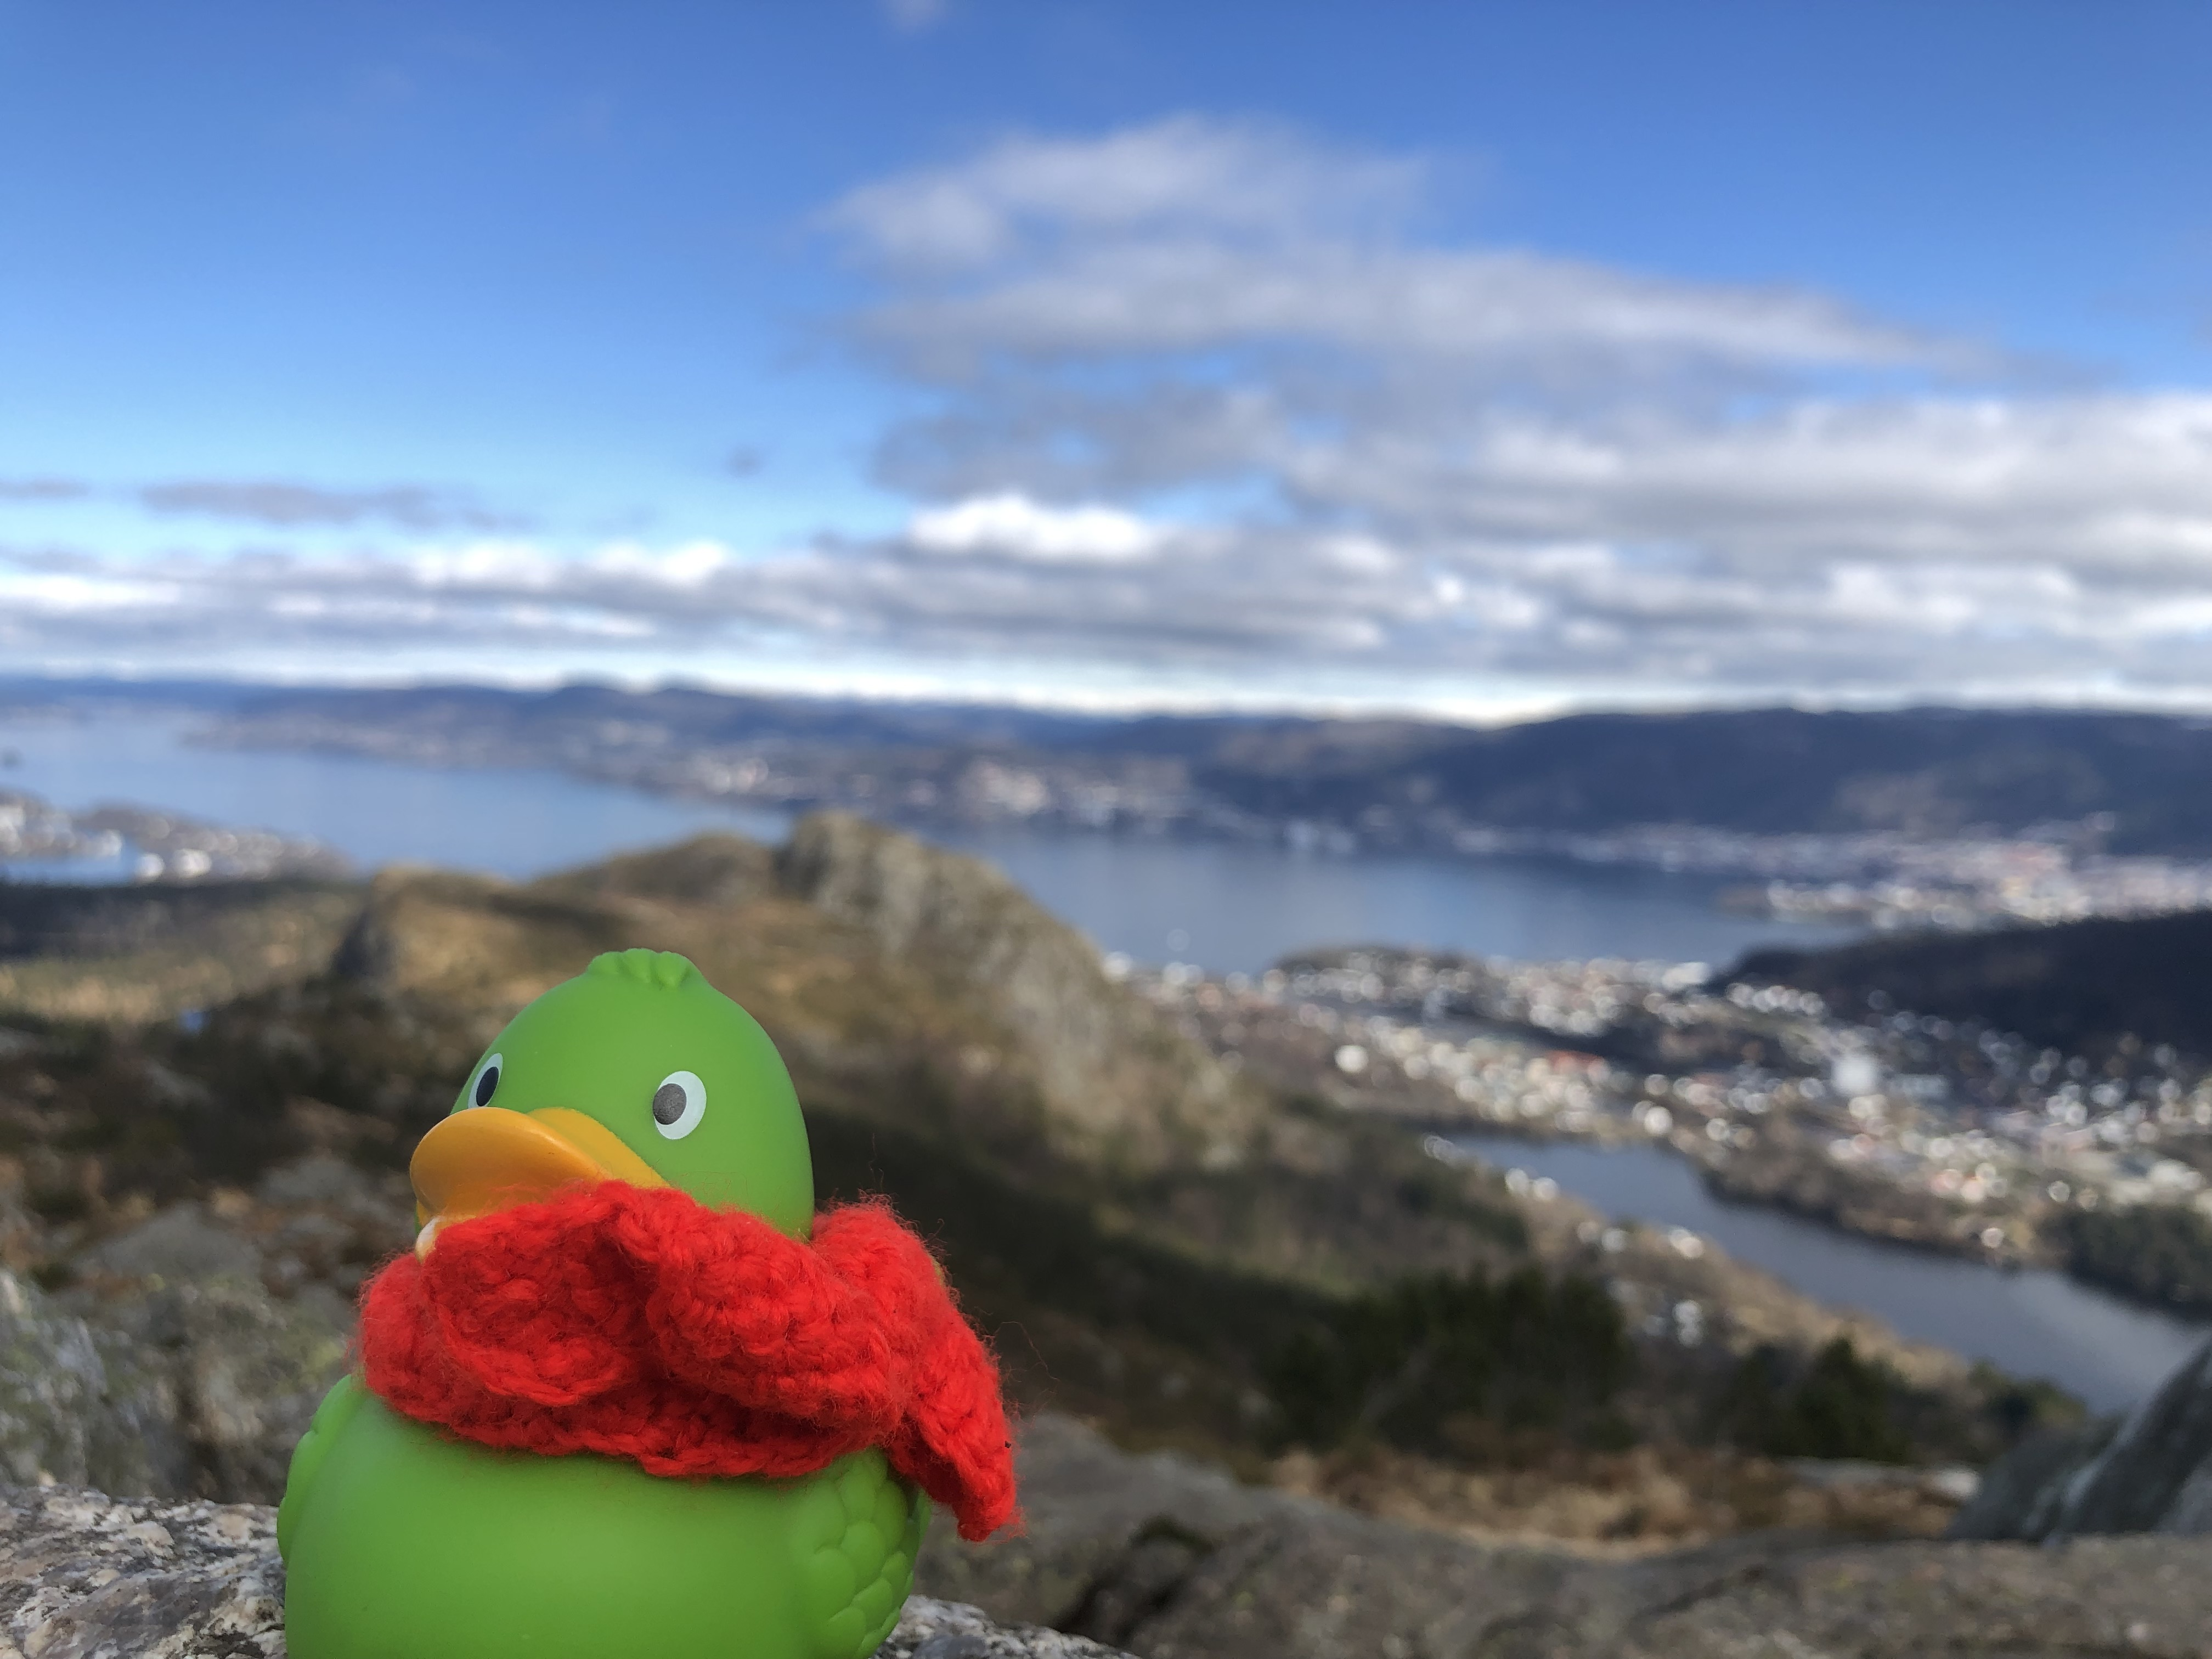
\includegraphics[height = 4.9cm]{images/guillaume8.jpg}
        \caption{Guillaume på Lyderhorn}
        \label{fig:guillaume8}
    \end{figure}
\end{frame}

% Frames sind nicht Gleichzusetzen mit Seiten
% Ein Frame kann aus mehreren Seiten bestehen
% Ein Frame repräsentiert das, was ein Mensch als eine Seite ansieht, getrennt durch Animationseffekte wie das Aufklappen von weiteren Inhalten
% Ein Frame mit nur einer Aufzählung, die aus vier Unterpunkten besteht, die sich einzeln ausklappen ist also ein Frame, bestehend aus vier Seiten

% Beamer hat ebenfalls Sections und Subsections
% Sections werden im Header oben angezeigt und mit der Anzahl von \textit{Frames} oben als Punkte repräsentiert
%\section{Sichtbarkeiten}
%\subsection{Aufzählungen}
%
%% Der zweite Befehl hinter Frame fügt einen Extratitel auf der Folie ein
%% Man kann ihn auch weglassen
%\begin{frame}{Aufzählungen: Automatisches Aufklappen}
%% [<+->] Lässt alles einzeln aufklappen
%% [<+(2)->] stellt alternativ die Schritthöhe um, im Beispiel für zwei Unterpunkte auf einmal
%\begin{itemize}[<+->]
%    \item Aufzählungen funktionieren wie in klassischem LaTeX
%    \item Man kann einstellen, dass jeder Unterpunkt einzeln aufgeklappt wird
%    \item Hierdurch erhält jeder Unterpunkt einen einzelnen Frame
%    \item Hierfür muss nur hinter itemize ein Aufklappbefehl eingefügt werden
%\end{itemize}
%
%\end{frame}
%
%% <1-> Wird in x-tem (hier 1) Teilframe mit ausgeklappt
%\begin{frame}{Aufzählungen: Explizites}
%\begin{itemize}
%    \item<1-> Es ist möglich hinter jeden item-Befehl zu notieren, in der wievielten Teilseite dieses Frames es mit aufgeklappt wird.
%    \item<2-> In diesem Beispiel wird Punkt 1 allein aufgeklappt
%    \item<2-> Punkt 2 und 3 jedoch gemeinsam
%    \item<3-> Dieser hier wieder allein
%\end{itemize}
%
%\end{frame}
%
%% Der <a-b>-Befehl hat einen zweiten Parameter, welcher sagt, wann etwas verschwinden soll, wenn die Folie noch nicht fertig ist
%\begin{frame}{Aufzählungen: Sichtbar <von – bis>}
%\begin{itemize}
%    \item<1-2> Der genannte Befehl lässt auch Text wieder verschwinden, bevor der Befehl vorbei ist
%    \item<2-> In diesem Beispiel wird 
%    \item<2-> der erste Satz mit dem offenbaren des letzten Unterpunkts verschwinden
%    \item<3-> Lasset Punkt 1 verschwinden!
%\end{itemize}
%
%\end{frame}
%
%% \pause führt zu einer "Aufklapppause" und alles danach ist in einer neuen Folie
%\begin{frame}{Aufzählungen: Pausenbefehl}
%\begin{itemize}
%    \item Es gibt auch einen \texttt{pause}-Befehl
%    \item Mit ihm wird alles bis zu einem bestimmten Punkt aufgeklappt
%    \pause
%    \item Und alles danach in eine neue Folie gepackt
%\end{itemize}
%
%\end{frame}
%
%\subsection{Weitere Übergänge}
%% Pause-Befehl auch für allgemeine Textabschnitte oder sonstigen Kram nutzbar
%\begin{frame}{Sichtbarkeit von Text}
%Der Pause-Befehl ermöglicht es auch jedwede weitere Sachen erst nach und nach erscheinen zulassen.\pause~Dies ist zum Beispiel bei Fließtext der Fall.
%% Hinweis: ~ hinter einem Befehl erzeugt ein Leerzeichen, weil LaTeX sonst keines einfügen würde
%\end{frame}
%
%% Der Visible-Befehl sagt an, auf welchen Folien etwas sichtbar sein soll (analog zu <a-b>)
%\begin{frame}{Der Visible-Befehl}
%Auch der von-bis-Befehl hat für beliebige Sachen ein Pendant. Man kann mit dem \texttt{Visible}-Befehl und geschwungenen Klammern einen Bereich umrahmen, der nur von Teil-Seite x bis y sichtbar sein wird.
%
%\newLine % Der NewLine-Befehl wurde in der Präambel definiert und ist kein LaTeX-Standard. Er führt zu einem angenehmen Zeilenumbruch, der für Zentrierung der Inhalte einer Folie führt
%\visible<2-3>{
% $ G := (V, E)$ with $V$ a set of vertices and $E := \{ (a, b)$ and $(b, a)$ with $a, b \in V $ and $ a \neq b \} $
%
%}
%    
%\visible<3-3>{
%  \newLine
%  $ G = (\{1, 2, 3, 4, 5, 6\}, \{(1, 2), (2, 1),
%      (1, 3), (3, 1),
%      (1, 4), (4, 1), 
%      (2, 4), (4, 2), $ \\
%  \quad\quad $ (2, 5), (5, 2),
%      (2, 6), (6, 2),
%      (3, 4), (4, 3),
%      (3, 6), (6, 3),
%      (5, 6), (6, 5)\}) $
%}
%
%\visible<4>{
%  \begin{center}
%    Ich lasse nun all den Mathekram verschwinden
%  \end{center}
%}
%\end{frame}
%
%
%% Der Only-Befehl funktioniert ähnlich wie visible, gibt jedoch den Platz wieder an das nächste Element zurück
%\begin{frame}{Der Only-Befehl}
%Der Only-Befehl funktioniert wie Visible, aber gibt den Platz wieder frei\\
%\begin{center}
%  \begin{tabular}{cccccc}
%    $ \begin{tabular}{c}1: \\2: \\3: \\4: \\5: \end{tabular} $ &
%    $ \begin{bmatrix}-1.28078 \\0.280776 \\-1 \\-1.28078 \\2.28078 \end{bmatrix} $ &
%    $\rightarrow$ &
%    $ \begin{bmatrix}-1 \\1 \\-1 \\-1 \\1 \end{bmatrix} $ &
%    \visible<2>{$\rightarrow$} &
%    \visible<2>{\noindent\parbox[c]{2.5cm}{ $V_1 = \{1,3,4\}\\V_2 = \{2,5,6\}$}}
%  \end{tabular}\\
%  % Anmerkung: Die Mathematik dieser Folie ist nicht korrekt und dient Anschauungszwecken
%  
%  \only<1>{% Graph 1 ist auf der ersten Folie sichtbar
%    \myGraph
%  }
%  \only<2>{% Graph 2 ist auf der nächsten Folie an seiner Stelle sichtbar
%    \myGraphCorrect
%  }
%\end{center}
%\end{frame}
%
%\section{Sonstiges}
%
%\subsection{Textblöcke}
%
%\begin{frame}
%    \frametitle{Textblöcke}
%    
%    Es gibt standardmäßig drei Sorten von Textblöcken in rot, grün und blau, die man sympathisch aussehend in Präsentationen einfügen kann. Ihre Farben sind wie in \LaTeX~ üblich änderbar und weitere hinzufügbar. Wenn man weiß wie. \alert{Ahahahamumumu}.
%    
%    % Der zweite Parameter (hier Remark) legt die Überschrift fest
%    \begin{block}{Remark}
%    Ihre Namen sind \texttt{block}, \texttt{alertblock} und \texttt{examples}
%    \end{block}
%    
%    \begin{alertblock}{Important theorem}
%    Französisch ist eine schrecklich anstrengende Sprache.
%    \end{alertblock}
%    
%    \begin{examples}
%    Un bel avion est un avion qui vole bien.
%    \end{examples}
%\end{frame}
%
%\subsection{Zweispaltiges Layout}
%\begin{frame}
%    \begin{columns}
%    
%    \column{0.5\textwidth}
%    Darstellung in zwei Spalten ist \textit{natürlich} möglich.
%    $$P\stackrel{?}{=} NP$$
%    \begin{itemize}
%    \item Präsentationsfanatiker können auch hier
%    \item die Spalten nacheinander erscheinen lassen
%    \item Aber wer macht sowas?
%    \end{itemize}
%    
%    \pause
%    \column{0.5\textwidth}
%    Hierfür nutzt man den \texttt{column}-Befehl und setzt die Breite der Columns entsprechend fest. Hier ist das eine 50-50-Aufteilung.
%    \end{columns}
%
%\end{frame}
%
%% Ein komplexeres Beispiel
%% noframenumbering führt dazu, dass eine Seite nicht mit in die Seitenzahlen hinein gezählt wird
%% Wer braucht sowas? Ingen vet
%\begin{frame}[noframenumbering]
% \begin{columns}
%    \begin{column}{0.52\textwidth}
%	\begin{table}
%    	\begin{tabular}{l|l|c|c|}
%    	\multicolumn{2}{c}{}&\multicolumn{2}{c}{Tatsächlich}\\
%    	\cline{3-4}
%    	\multicolumn{2}{c|}{}&Positiv&Negativ\\
%    	\cline{2-4}
%    	\multirow{2}{*}{Vorhergesagt}& Positiv & $TP$ & $FP$\\
%    	\cline{2-4}
%    	& Negativ & $FN$ & $TN$\\
%    	\cline{2-4}
%    	\end{tabular}
%	    \caption{Konfusionsmatrix}
%	    \label{tab:confusion-matrix}
%    \end{table}
%    \end{column}
%    
%    \begin{column}{0.52\textwidth}
%    \begin{center}
%        ${\displaystyle Precision = \frac{TP}{TP+FP} } $\\[5mm]
%        ${\displaystyle Recall = \frac{TP}{TP+FN} } $\\[5mm]
%        ${\displaystyle F_1 = \frac{2\cdot Precision\cdot Recall}{Precision + Recall} } $
%    \end{center}
%    \end{column}
% \end{columns}
%\end{frame}
%
%\subsection{Bilder einfügen}
%\begin{frame}{Graphiken einfügen wie sonst auch}
%    \begin{figure}
%        \centering
%        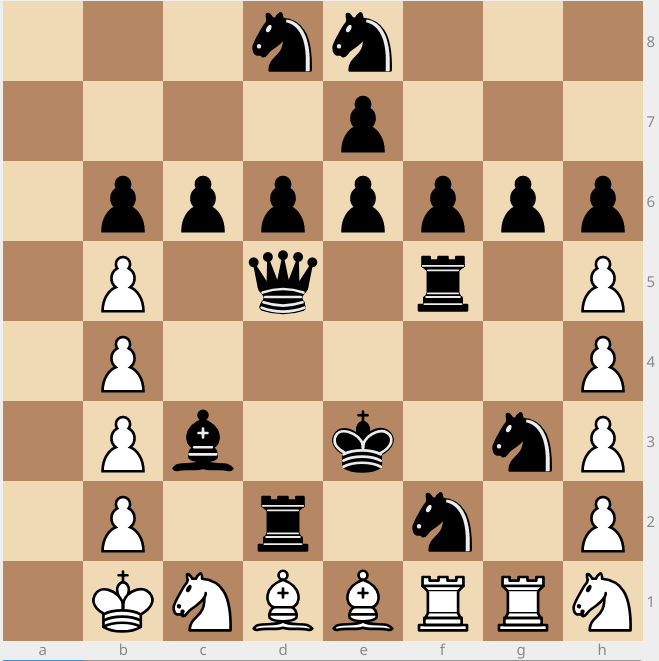
\includegraphics[height = 4.9cm]{puzzle.png}
%        \caption{Schwarz am Zug, Matt in 5}
%        \label{fig:chesspuzzle}
%    \end{figure}
%\end{frame}


\section*{Slutt}
\begin{frame}
\begin{center}
\begin{Large}
\textbf{Takk for oppmerksamheten\\[5mm]
Lykke til med eksamenen}
\end{Large}
\end{center}  
\end{frame}